
% XXX- discuss GtkBin; which widgets have a window, which do not --image and label do not, and we mightwant them too,
%   modify_bg() only affects widgets that have an associated gtk.gdk.Window.
% > Widgets that do not have an associated window include .... gtk.Arrow,
% > gtk.Bin, gtk.Box, gtk.Button, gtk.CheckButton, gtk.Fixed , gtk.Image ,
% > gtk.Label , gtk.MenuItem , gtk.Notebook , gtk.Paned , gtk.RadioButton ,
% > gtk.Range , gtk.ScrolledWindow , gtk.Separator , gtk.Table , gtk.Toolbar ,
% > gtk.AspectFrame , gtk.Frame , gtk.VBox , gtk.HBox , gtk.VSeparator ,
% > gtk.HSeparator . These widgets can be added to a gtk.EventBox to overcome
% > this limitation.




%% RGtk2 chapter
\chapter{RGtk2: Overview}
%%\section{Introduction}
\label{sec:RGtk2-Introduction}
%% intorduction

%% Technical, but short beginning

As the name implies, the \pkg{RGtk2} package is an interface, or
binding, between \R\/ and \GTK, a mature, cross-platform GUI
toolkit. The letters \emph{GTK} stand for the \emph{GIMP ToolKit},
with the word \emph{GIMP} recording the origin of the library as part
of the GNU Image Manipulation Program. \pkg{GTK+} provides the same
widgets on every platform, though it can be customized to emulate
platform-specific look and feel. The library is written in
\proglang{C}, which facilitates access from languages like
\proglang{R} that are also implemented in \proglang{C}. \pkg{GTK+} is
licensed under the \textit{Lesser GNU Public License} (LGPL), while
\pkg{RGtk2} is under the \textit{GNU Public License} (GPL).
The package is available from the Comprehensive \proglang{R} Archive
Network (CRAN) at \url{http://CRAN.R-project.org/package=RGtk2}.

The name \pkg{RGtk2} also implies that there exists a package named
\pkg{RGtk}, which is indeed the case. The original \pkg{RGtk} is bound
to the previous generation of \pkg{GTK+}, version 1.2. \pkg{RGtk2} is
based on \pkg{GTK+ 2.0}, the current generation. This book covers
\pkg{RGtk2} specifically, although many of the fundamental features of
\pkg{RGtk2} are inherited from \pkg{RGtk}. 

\pkg{RGtk2} provides virtually all of the functionality in \GTK\/ to
the \R\/ programmer. In addition, \pkg{RGtk2} interfaces with several
other libraries in the \GTK\/ stack: Pango for font rendering; Cairo
for vector graphics; GdkPixbuf for image manipulation; libglade for
designing GUI layouts from an XML description; ATK for accessible
interfaces; and GDK, an abstraction over the native windowing system,
supporting either X11 or Windows. These libraries are multi-platform
and extensive and have been used for many major projects, such as the
Linux versions of Firefox and Open Office.

The API of each of these libraries is mapped to \R\/ in a way that is
consistent with \R\/ conventions and familiar to the \R\/
user. Much of the \pkg{RGtk2} API consists of autogenerated \R\/
functions that call into the one of the underlying libraries. For
example, the \R\/ function \function{gtkContainerAdd} eventually calls
the C function \code{gtk\_container\_add}. The naming convention is
that the C name has its underscores removed and each following letter
capitalized (camelback style).

The full API for \GTK\/ is quite large, and complete documentation of
it is beyond our scope. However, the \GTK\/ documentation is
algorithmically converted into the \R\/ help format during the
generation of \pkg{RGtk2}. This conveniently allows the programmer to
refer to the appropriate documentation within an \R\/ session, without
having to consult a web page, such as
\url{http://library.gnome.org/devel/gtk/stable/}, which lists the
\proglang{C} API of the stable versions \GTK.

In this chapter, we give an overview of how \pkg{RGtk2} maps the
\GTK\/ API, including its classes, constructors, methods, properties,
signals and enumerations, to an \R-level API that is relatively
familiar to and convenient for an \R\/ user. A simple GUI will be
gradually constructed to demonstrate the API.

%%% ------- OOP --------------

\section{Objects and Classes}

In any toolkit, all widget types have functionality in common. For
example, they are all drawn on the screen in a consistent style. They
can be hidden and shown again. To formalize this relationship and to
simplify implementation by sharing code between widgets, \pkg{GTK+},
like many other toolkits, defines an inheritance hierarchy for its
widget types. In the parlance of object-oriented programming, each
type is represented by a \textit{class}.

For specifying the hierarchy, \pkg{GTK+} relies on \pkg{GObject}, a
\proglang{C} library that implements a class-based, single-inheritance
object-oriented system. A \pkg{GObject} class encapsulates behaviors
that all instances of the class share. Every class has at most one
parent from which it inherits the behaviors of its ancestors. A
subclass can override some specific inherited behaviors. The interface
defined by a class consists of constructors, methods, properties,
and signals. 
% TODO: example of gTypeGetAncestors

Single inheritance can be restrictive when a class performs multiple
roles in a program. To circumvent this, \pkg{GTK+} adopts the popular
concept of the \textit{interface}, which is essentially a contract
that specifies which methods, properties and signals a class must
implement. As with languages like Java and C#, a class can
\textit{implement} multiple interfaces, and an interface can be
composed of other interfaces. An interface allows the programmer to
treat all instances of implementing classes in a similar way. However,
unlike class inheritance, the implementation of the methods,
properties and signals is not shared.
% TODO: example of gTypeGetInterfaces

We explain the constructors, methods, properties and signals of
classes and interfaces in the following sections and demonstrate them
in the construction of a simple ``Hello World'' GUI, shown in
Figure~\ref{fig:hello-world}. A more detailed and technical
explanation of \pkg{GObject} is available in
Section~\ref{sec:gobject-primer}.

\begin{figure}[h!tbp]
  \begin{center}
    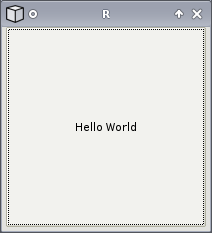
\includegraphics[width=2in]{hello-world.png}
    \caption{\label{fig:hello-world}``Hello World'' in GTK+. 
      A window containing a single button displaying a label with the text
      \code{Hello World}.}
  \end{center}
\end{figure}

\section{Constructors}

The first step in our example is to create a top-level window to
contain our GUI.  Creating an instance of a GTK\/ widget requires
calling a single \R\/ function, known as a constructor. Following \R\/
conventions, the constructor for a class has the same name as the
class, except the first character is lowercase. The following
statement constructs an instance of the \code{GtkWindow} class:
\begin{Schunk}
\begin{Sinput}
 window <- gtkWindow("toplevel", show = FALSE)
\end{Sinput}
\end{Schunk}
%
The first argument to the constructor for \code{GtkWindow} instructs
the window manager to treat the window as top-level.  The \code{show}
argument is the last argument for every widget constructor. It
indicates whether the widget should be made visible immediately after
construction.  The default value of \code{show} is \code{TRUE}. In
this case we want to defer showing the window until after we finish
constructing our simple GUI.

At the \GTK\/ level, a class usually has multiple constructors, each
implemented as a separate C function. In \pkg{RGtk2}, the names of
these functions all end with \code{New}. The ``meta'' constructor
\function{gtkWindow}, called above, automatically delegates to one of
the low-level constructors, based on the provided arguments.

A \GTK\/ object created by the \R\/ user has an \R-level object as its
proxy. Thus, \code{window} is a reference to a \class{GtkWindow}
instance.  The class hierarchy of a proxy object is represented by the
\code{class} attribute. One interprets the attribute according to S3
conventions, so that the class names are in order from most to least
derived:
\begin{Schunk}
\begin{Sinput}
 class(window)
\end{Sinput}
\begin{Soutput}
[1] "GtkWindow"         "GtkBin"            "GtkContainer"     
[4] "GtkWidget"         "GtkObject"         "GInitiallyUnowned"
[7] "GObject"           "RGtkObject"       
\end{Soutput}
\end{Schunk}
%
We find that the \class{GtkWindow} class inherits methods,
properties, and signals from the \class{GtkBin}, \class{GtkContainer},
\class{GtkWidget}, \class{GtkObject}, \class{GInitiallyUnowned}, and
\class{GObject} classes. Every type of \pkg{GTK+} widget inherits from
the base \code{GtkWidget} class, which implements the general
characteristics shared by all widget classes, e.g., properties storing
the location and background color; methods for hiding, showing and
painting the widget. We can also query \code{window} for the
interfaces it implements:
\begin{Schunk}
\begin{Sinput}
 interface.GObject(window)
\end{Sinput}
\begin{Soutput}
[1] "AtkImplementorIface" "GtkBuildable"       
\end{Soutput}
\end{Schunk}

When the underlying \GTK\/ object is destroyed, i.e., deleted
from memory, the class of the proxy object is set to \class{<invalid>},
indicating that it can no longer be manipulated.

\section{Methods}

The next steps in our example are to create a ``Hello World'' button
and to place the button in the window that we have already
created. This depends on an understanding of how of one
programmatically manipulates widgets by invoking methods.  Methods are
functions that take an instance of their class as the first argument
and instruct the widget to perform an action.

Although class information is stored in the style of S3, \pkg{RGtk2}
introduces its own mechanism for method dispatch.  The call
\code{obj\$method(...)}  resolves to a function call
\code{f(obj,...)}. The function is found by looking for any function
that matches the pattern \emph{classNameMethodName}, the concatenation
of one of the names from \code{class(obj)} or \code{interface(obj)}
with the method name. The search begins with the interfaces and
proceeds through each character vector in order.

For instance, if \code{win} is a \function{gtkWindow} instance, then
to resolve the call \code{win\$add(widget)} \pkg{RGtk2} considers
\function{gtkBuildableAdd}, \function{atkImplementorIfaceAdd},
\function{gtkWindowAdd}, \function{gtkBinAdd} and finally finds
\function{gtkContainerAdd}, which is called as
\code{gtkContainerAdd(win, widget)}. The \method{\$}{GObject} method
for \pkg{RGtk2} objects does the work.

We take advantage of this convenience when we add the ``Hello World''
button to our window and set its size:
\begin{Schunk}
\begin{Sinput}
 button <- gtkButton("Hello World")
 window$add(button)
 window$setDefaultSize(200, 200)
\end{Sinput}
\end{Schunk}
%
The above code calls the \function{gtkContainerAdd} and
\function{gtkWindowSetDefaultSize} functions with less typing and less
demands on the memory of the user.

Understanding this mechanism allows us to add to the \pkg{RGtk2}
API. For instance, we can add to the button API with
\begin{Schunk}
\begin{Sinput}
 gtkButtonSayHello <- function(obj, target) 
   obj$setLabel(paste("Hello", target))
 button$sayHello("John")
 button$getLabel()
\end{Sinput}
\begin{Soutput}
[1] "Hello John"
\end{Soutput}
\end{Schunk}

%% common methods
Some common methods are inherited by most widgets, as they are defined
in the base \class{gtkWidget} class. These include the methods 
\method{show}{gtkWidget} to specify that the widget should be drawn;
\method{hide}{gtkWidget} to hide the widget until specified;
\method{destroy}{gtkWidget} to destroy a widget and clear up any
references to it; \method{getParent}{gtkWidget} to find the parent
container of the widget; \method{modifyBg}{gtkWidget} to modify the
background color of a widget; and \method{modifyFg}{gtkWidget} to
modify the foreground color.


\section{Properties}


%% --------- Properties ------------
The \GTK\/ API uses properties to store object state. Properties are
similar to \R\/ attributes and even more so to S4 slots. They are
inherited, typed, self-describing and encapsulated, so that an object
can intercept access to the underlying data. A list of properties that
a widget has is returned by its \method{getPropInfo}{GObject}
method. \pkg{RGtk2} provides the \R\/ generic \method{names}{GObject}
as a familiar alternative for this method. Auto-completion of property
names is gained as a side effect.  For the button just defined, we can
see the first eight properties listed with:
\begin{Schunk}
\begin{Sinput}
 head(names(button), n=8)                     # or b$getPropInfo()
\end{Sinput}
\begin{Soutput}
[1] "user-data"      "name"           "parent"         "width-request" 
[5] "height-request" "visible"        "sensitive"      "app-paintable" 
\end{Soutput}
\end{Schunk}

Some common properties are: \code{parent}, to store the parent widget
(if any); \code{user-data}, which allows one to store arbitrary data
with the widget; and \code{sensitive}, to control whether a widget can
receive user events. 

There are a few different ways to access these properties. \GTK\/
provides the functions \function{gObjectGet} and \function{gObjectSet}
to get and set properties of a widget. The set funtion treats the
arguments names as the property names, and setting multiple properties
at once is supported. Here we add an icon to the top-left corner of
our window and set the title:
\begin{Schunk}
\begin{Sinput}
 image <- gdkPixbuf(filename = imagefile("rgtk-logo.gif"))[[1]]
 window$set(icon = image, title = "Hello World 1.0")
\end{Sinput}
\end{Schunk}

Additionally, most user-accessible properties have specific \code{get} and
\code{set} methods defined for them. For example, to set the title of
the window, we could have used the \method{setTitle}{GtkWindow} method
and verified the change with \method{getTitle}{GtkWindow}.
\begin{Schunk}
\begin{Sinput}
 window$setTitle("Hello World 1.0")
 window$getTitle()
\end{Sinput}
\begin{Soutput}
[1] "Hello World 1.0"
\end{Soutput}
\end{Schunk}

\pkg{RGtk2} provides the convenient and familiar \code{[} and
\code{[$<$-} methods to get and access the properties. In our example,
we might check the window to ensure that it is not yet visible:
\begin{Schunk}
\begin{Sinput}
 window["visible"]
\end{Sinput}
\begin{Soutput}
[1] FALSE
\end{Soutput}
\end{Schunk}
Finally, we can make our window visible by setting the ``visible'' property,
although calling \function{gtkWidgetShow} is more conventional:
\begin{Schunk}
\begin{Sinput}
 window["visible"] <- TRUE 
 window$show() # same effect
\end{Sinput}
\end{Schunk}

For ease of referencing the appropriate help pages, we tend to use the
full method name in the examples, although at times the move \R-like
vector notation will be used for commonly accessed properties.

%%% ------ Signals ----------

\section{Events and signals}

In \pkg{RGtk2}, a user action, such as a mouse click, key press, or
drag and drop motion, triggers the widget to emit a corresponding
signal.  A GUI can be made interactive by specifying a callback
function to be invoked upon the emission of a particular signal.

The signals provided by a class or interface are returned by the
function \function{gTypeGetSignals}. For example
\XXX{JV: comment out until upgrade to RGtk2}
\begin{Schunk}
\begin{Sinput}
 names(gTypeGetSignals("GtkButton"))
\end{Sinput}
\end{Schunk}
shows the ``clicked'' signal in addition to others. Note that this
only lists the signals provided directly by the \class{GtkButton}. To
list all inherited signals, we need to loop over the hierarchy, but it
is not common to do this in practice, as the documentation includes
information on the signals.

The \function{gSignalConnect} (or \function{gSignalConnect}) function is used
to add a callback to a widget's signal. Its signature is
\begin{Schunk}
\begin{Sinput}
 args(gSignalConnect)
\end{Sinput}
\begin{Soutput}
function (obj, signal, f, data = NULL, after = FALSE, user.data.first = FALSE)  
\end{Soutput}
\end{Schunk}
%
The basic usage is to call \function{gSignalConnect} to connect a
callback function \argument{f}{gSignalConnect} to the signal named
\argument{signal}{gSignalConnect} belonging to the object
\argument{obj}{gSignalConnect}. The function returns an identifier for
managing the connection. This is not usually necessary but will be
discussed later.

We demonstrate this usage by adding a callback to our ``Hello World''
example, so that ``Hello World'' is printed to the console when the
button is clicked:
\begin{Schunk}
\begin{Sinput}
 gSignalConnect(button, "clicked", 
                function(widget) print("Hello world!"))
\end{Sinput}
\begin{Soutput}
clicked 
     12 
attr(,"class")
[1] "CallbackID"
\end{Soutput}
\end{Schunk}
%

The \argument{data}{gSignalConnect} argument allows arbitrary data to
be passed to the callback.  The
\argument{user.data.first}{gSignalConnect} argument specifies if this
\argument{data}{gSignalConnect} argument should be the first argument
to the callback or (the default) the last.

The \argument{after}{gSignalConnect} argument is a logical indicating
if the callback should be called after the default handlers (see
\command{?gSignalConnect}).

%% the callback
The signature for the callback varies for each signal. Unless
\code{user.data.first} is \code{TRUE}, the first argument is the
widget. Other arguments are possible depending on the signal type. For
window events, the second argument is a \class{GdkEvent} type, which
can carry with it extra information about the event that occurred. The
\GTK\/ API lists the signature of each signal.

Is important to note that the widget, and possibly other arguments,
are references, so their manipulation has side effects outside of the
callback. This is obviously a critical feature, but it is one that
may be surprising to the \R\/ user.

\begin{Schunk}
\begin{Sinput}
 w <- gtkWindow(); w['title'] <- "test signals"
 x <- 1; 
 b <- gtkButton("click me"); w$add(b)
 ID <- gSignalConnect(b, signal = "clicked", f = function(widget) {
   widget$setData("x", 2)
   x <- 2
   return(TRUE)
 })
\end{Sinput}
\end{Schunk}
Then after clicking, we would have

\begin{Schunk}
\begin{Sinput}
 cat(x, b$getData("x"), "\n") # 1 and 2
\end{Sinput}
\begin{Soutput}
1 2 
\end{Soutput}
\end{Schunk}

Callbacks for signals emitted by window manager events are expected to
return a logical value. Failure to do so can cause errors to be
raised. For most other callbacks the return value is ignored, so it is
safe to always return a logical value. For window events, a
return value of \code{TRUE} indicates that no further
callbacks should be called, whereas \code{FALSE} indicates that the
next callback should be called. So in the following example, only the
first two callbacks are executed when the user presses on the button.

\begin{Schunk}
\begin{Sinput}
 b <- gtkButton("click")
 w <- gtkWindow()
 w$add(b)
 id1 <- gSignalConnect(b, "button-press-event", 
 function(b, event, data) {
   print("hi"); return(FALSE)
 })
 id2 <- gSignalConnect(b, "button-press-event", 
 function(b, event, data) {
   print("and"); return(TRUE)
 })
 id3 <- gSignalConnect(b, "button-press-event", 
 function(b, event, data) {
   print("bye"); return(TRUE)
 })
\end{Sinput}
\end{Schunk}

%% multiple callbacks; remove; block
Multiple callbacks can be assigned to each signal. They will be
processed in the order they were bound to the signal.  The
\function{gSignalConnect} function returns an ID that can be used to
disconnect a callback if desired using
\function{gSignalHandlerDisconnect} or temporarily blocked using
\function{gSignalHandlerBlock} and
\function{gSignalHandlerUnblock}. The man page for
\function{gSignalConnect} gives the details on this, and much more.

%%% ------ constants --------

\section{Enumerated types and flags}

At the beginning of our example, we constructed the window thusly: 
\begin{Schunk}
\begin{Sinput}
 window <- gtkWindow("toplevel", show = FALSE)
\end{Sinput}
\end{Schunk}
%
The first parameter indicates the window type. The set of possible
window types is specified by what in \proglang{C} is known as an
\emph{enumeration}. A value from an enumeration can be thought of as a
length one factor in \R. The possible values defined by the
enumeration are analogous to the factor levels.  Since enumerations
are foreign to \proglang{R}, \pkg{RGtk2} accepts string
representations of enumeration values, like \code{"toplevel"}. 

For every \pkg{GTK+} enumeration, \pkg{RGtk2} provides an \proglang{R}
vector that maps the nicknames to the underlying numeric values.  In
the above case, the vector is named \code{GtkWindowType}.
\begin{Schunk}
\begin{Sinput}
 GtkWindowType
\end{Sinput}
\begin{Soutput}
toplevel    popup 
       0        1 
attr(,"class")
[1] "enums"
\end{Soutput}
\end{Schunk}
%
The names of the vector indicate the allowed nickname for each value
of the enumeration. It is rarely necessary to explicitly use the
enumeration vectors; specifying the nickname will work in most cases,
including all method invocations, and is preferable as it is easier
for human readers to comprehend.

Flags are an extension of enumerations, where the value of each member
is a unique power of two, so that the values can be combined
unambiguously. An example of a flag enumeration is
\class{GtkWidgetFlags}.
\begin{Schunk}
\begin{Sinput}
 GtkWidgetFlags
\end{Sinput}
\begin{Soutput}
        toplevel        no-window         realized           mapped 
              16               32               64              128 
         visible        sensitive parent-sensitive        can-focus 
             256              512             1024             2048 
       has-focus      can-default      has-default         has-grab 
            4096             8192            16384            32768 
        rc-style  composite-child      no-reparent    app-paintable 
           16384           131072           262144           524288 
receives-default  double-buffered      no-show-all 
         1048576          2097152          4194304 
attr(,"class")
[1] "flags"
\end{Soutput}
\end{Schunk}
%
\class{GtkWidgetFlags} represents the possible flags that can be set
on a widget. We can retrieve the flags currently set on our window:
\begin{Schunk}
\begin{Sinput}
 window$flags()
\end{Sinput}
\begin{Soutput}
[1] 2164688
attr(,"class")
[1] "GtkWidgetFlags" "flag"          
\end{Soutput}
\end{Schunk}
%
Flag values can be combined using \function{|}, the bitwise
\textit{OR}. The \function{\&} function, the bitwise \textit{AND},
allows one to check whether a value belongs to a combination. For
example, we could check whether our window is top-level:
\begin{Schunk}
\begin{Sinput}
 (window$flags() & GtkWidgetFlags["toplevel"]) > 0
\end{Sinput}
\begin{Soutput}
[1] TRUE
\end{Soutput}
\end{Schunk}

%% --------- Event Loop

\section{The event loop}


\pkg{RGtk2} integrates the \GTK\/ eventloop with the \R\/ event
loop. A separate thread continuously iterates the \GTK\/ event loop,
in synchronization with the main \R\/ thread.  Thus, if the \R\/
thread is busy, the \GTK\/ event loop will not be iterated. During a
long calculation, the GUI can seem unresponsive. To avoid this, the
following construct should be inserted into the long running algorithm
in order to ensure that \GTK\/ events are periodically processed.

\begin{Schunk}
\begin{Sinput}
 while(gtkEventsPending()) 
   gtkMainIteration()
\end{Sinput}
\end{Schunk}


%% MOVEME: seems like integration between gWidgets and native toolkits
%% belongs in the gWidgets chapters. Otherwise, each toolkit chapter
%% needs to say the same thing. Better to have it in one place.

% \section{RGtk2 and gWidgetsRGtk2}
% \label{sec:RGtk2:gWidgetsRGtk2}


% The widgets described above, are also available through
% \pkg{gWidgetsRGtk2}. The two packages can be used together, for the
% most part. The \code{add} method of \pkg{gWidgetsRGtk2} can be used to
% add an \pkg{RGtk2} widget to a \code{gWidgetsRGtk2}
% container. Whereas, the \code{getToolkitWidget} method will (usually)
% return the \pkg{RGtk2} component to use within \pkg{RGtk2}.

%% Views example in next chapter?

\chapter{RGtk2: Basic Components}
\label{sec:top-level-windows}

\XXX{ --- GDkWindow role (events, coloring, event box): explain on need
to know basis}

\XXX{SetDecorated for gtkWindow}


This section covers some of the basic widgets and containers of
\GTK. We begin with a discussion of top level containers and box
containers. Then we describe many of the basic controls, and
conclude with the mention of a few special-case containers.

\section{Top-level windows}
\label{sec:RGtk2:gtkWindow}

%% constructor Show/Hide
As we saw in our ``Hello World'' example, top-level windows are
constructed by the \constructor{gtkWindow} constructor. This function
has arguments \code{type} to specify the type of window to create. The
default is a top-level window, which we will always use, as the
alternative is for ``popups'' which are meant for internal use, e.g.,
for implementing menus. The second argument is \code{show}, which by
default is \code{TRUE}, indicating that the window should be shown. If
set to \code{FALSE}, the window, like other widgets, can later be
shown by calling its \method{show}{gtkWidget} method. The
\method{showAll}{gtkWidget} method will also show any child
components. These can be reversed with \method{hide}{gtkWidget} and
\method{hideAll}{gtkWidget}.

%% title
As with all objects, windows have several properties. The window title
is stored in the \code{title} property. As usual, this property can be
accessed via the ``get'' and ``set'' methods
\method{getTitle}{gtkWindow} and \method{setTitle}{gtkWindow}, or
using the \function{[} function. To illustrate, the following sets up
a new window with a title.
\begin{Schunk}
\begin{Sinput}
 w <- gtkWindow(show=FALSE)              # use default type
 w$setTitle("Window title")              # set window title
 w['title']                              # or w$getTitle()
\end{Sinput}
\begin{Soutput}
[1] "Window title"
\end{Soutput}
\begin{Sinput}
 w$setDefaultSize(250,300)               # 250 wide, 300 high
 w$show()                                # show window
\end{Sinput}
\end{Schunk}

\paragraph{Window size}
The initial size of the window can be set with the
\method{setDefaultSize}{gtkWindow} method, as shown, which takes a
\argument{width}{gtkWindow} and \argument{height}{gtkWindow} argument
specified in pixels. This specification allows the window to be
resized, but must be made before the window is drawn, as the window
then falls under control of the window manager. The
\method{setSizeRequest}{gtkWidget} method will request a minimum size,
which the window manager will usually honor, as long as a maximum
bound is not violated. To fix the size of a window, the
\code{resizable} property may be set to \code{FALSE}.

%% A container
\paragraph{Adding a child component to a window}
A window is a container. \class{GtkWindow} inherits from
\class{GtkBin}, which can contain only a single child. As before, this
child is added by the \method{add}{gtkContainer} method. To display
multiple widgets in a window, one simply needs to add a
non-\class{GtkBin} container as the child widget.

We illustrate the basics by adding a simple label to a window.
\begin{Schunk}
\begin{Sinput}
 w <- gtkWindow(show=FALSE); w$setTitle("Hello world")
 l <- gtkLabel("Hello world")
 w$add(l)
\end{Sinput}
\end{Schunk}
%

%% delete-event; destroy
\paragraph{Destroying windows}
A window is normally closed by the window manager. Most often, this
occurs in response to the user clicking on a close button in a title
bar. It is also possible to close a window programatically by calling
its \method{destroy}{gtkWidget} method. When the user clicks on the
close button, the window manager requests that the window be deleted,
and the \code{delete-event} signal is emitted.  The contract of
deletion is that the window should no longer visible on the screen. It
is not necessary for the actual window object to be removed from
memory, although this is the default behavior. Calling the
\code{hideOnDelete} method configures the window to hide but not
destroy itself. As with any event, the default handler is overridden
if a callback connected to \code{delete-event} returns \code{TRUE}.
This can be useful for confirming the intention of the user before
closing the window.

\paragraph{Transient windows}
New windows may be standalone top-level windows, or may be associated
with some other window. For example, a dialog is usually associated
with the primary document window. The
\method{setTransientFor}{gtkWindow} method can be used to specify the
window with which a transient (dialog) window is associated. This
hints the window manager that the transient window should be kept on
top of its parent. The position relative to the parent window can be
specified with \code{setPostion}, which takes a value from the
\code{GtkWindowPosition} enumeration. Optionally, a dialog be can be
set to be destroyed with its parent. For example:
\begin{Schunk}
\begin{Sinput}
 ## create a window and a dialog window
 w <- gtkWindow(show=FALSE); w$setTitle("Top level window")
 d <- gtkWindow(show=FALSE); d$setTitle("dialog window")
 d$setTransientFor(w)
 d$setPosition(GtkWindowPosition["center-on-parent"])
 d$setDestroyWithParent(TRUE)
 w$show()
 d$show()
\end{Sinput}
\end{Schunk}
% 
The above code produces a non-modal dialog window from scratch. Due to
its transient nature, it can hide parts of the top-level window, but,
unlike a modal dialog, it does not prevent that window from receiving
events. \GTK\/ provides a number of convenient high-level dialogs,
discussed later, that support modal operation.

%% ML: This seems like a natural place to treat dialogs.
%% Why leave them until the end? They are important to most any GUI.

% ML: I think it's better to talk about containers and layout all in
% one place. If a container is not often used, then less detail should
% be given, but it should still be described here.

\section{Layout containers}
\label{sec:RGtk2:layout}

Once a top-level window is constructed, it remains to fill the window
with the controls that will constitute our GUI. As these controls are
graphical, they must occupy a specific region on the screen. The
region could be specified explicitly, as a rectangle. However, as a
user interface, a GUI is dynamic and interactive. The size constraints
of widgets will change, and the window will be resized. The programmer
cannot afford to explicitly manage a dynamic layout. Thus, \GTK\/
implements automatic layout in the form of container widgets.

\subsection{Basics}
\label{sec:RGtk2:layout:basics}

The method \method{getChildren}{GtkContainer} will return the children
of a container as a list. Since in this case the list will be at most
length one, the \method{getChild}{GtkWidget} method may be more
convenient, as it directly returns the only child, if any. For
instance, to retrieve the label text one could do:
\begin{Schunk}
\begin{Sinput}
 w$getChild()['label']                   # return label property of child
\end{Sinput}
\begin{Soutput}
NULL
\end{Soutput}
\end{Schunk}


%% [[ for container
The \method{[[}{GObject} method 
%% ]]
accesses the child containers by number, as a convenient wrapper
around the \method{getChildren}{GObject} method. 

In \GTK{}, the widget hierarchy is built when children are added to a
parent container.  In our example, the window is the immediate parent
of the label. The \code{getParent} method for \GTK\/ widgets will
return the parent container of a widget.

Every container supports removing a child with the
\method{remove}{gtkWidget} method. The child can later be re-added
using \method{packStart}{gtkBox}. For instance
\begin{Schunk}
\begin{Sinput}
 b <- g[[3]]
 g$remove(b)                             # removed
 g$packStart(b, expand=TRUE, fill=TRUE)
\end{Sinput}
\end{Schunk}
% 
To remove a widget from the screen but not its container, use the
\method{hide}{gtkWidget} method on the widget. This can be reversed
with the \method{show}{gtkWidget} method. The
\method{reparent}{gtkWidget} method is a convenience for moving a
widget between containers.

\subsection{Widget size negotiation}
\label{sec:RGtk2:layout:size}

We have already seen perhaps the simplest automatic layout container,
\class{GtkWindow}, which fills all of its space with its child. While
simple, there is a considerable amount of logic for calculating the
size of the widget on the screen. The child will first inform the
parent of its desired natural size. For example, a label might ask for
the dimensions necessary to display all of its text. The container
then decides whether to allocate the requested size or to allocate
more or less than the requested amount. The child consumes the
allocated space. Consider the previous example of adding a label to a
window:
\begin{Schunk}
\begin{Sinput}
 w <- gtkWindow(show=FALSE); w$setTitle("Hello world")
 l <- gtkLabel("Hello world")
 w$add(l)
\end{Sinput}
\end{Schunk}
%
The window is shown before the label is added, and the default size is
likely much larger than the space the label needs to display ``Hello
world''. However, as the window size is now controlled by the window
manager, \class{GtkWindow} will not adjust its size. Thus, the label
is allocated more space than it requires.
\begin{Schunk}
\begin{Sinput}
 l$getAllocation()
\end{Sinput}
\begin{Soutput}
$x
[1] -1

$y
[1] -1

$width
[1] 1

$height
[1] 1

attr(,"class")
[1] "GtkAllocation"
\end{Soutput}
\end{Schunk}
%
If, however, we avoid showing the window until the label is added, the
window will size itself so that the label has its natural size:
\begin{Schunk}
\begin{Sinput}
 w <- gtkWindow(show=FALSE); w$setTitle("Hello world")
 l <- gtkLabel("Hello world")
 w$add(l)
 w$show()
 l$getAllocation()
\end{Sinput}
\begin{Soutput}
$x
[1] 0

$y
[1] 0

$width
[1] 79

$height
[1] 18

attr(,"class")
[1] "GtkAllocation"
\end{Soutput}
\end{Schunk}
%
One might notice that it is not possible to decrease the size of the
window further. This is due to \class{GtkLabel} asserting a minimum
size request that is sufficient to display its text. The
\method{setSizeRequest}{GtkWidget} sets a user-level minimum size 
request for any widget. It is obvious from the method name, however,
that this is still strictly a request. It may not be satisfied, for
example, if the maximum window size constraint of the window manager
is violated. More importantly, setting a minimum size request is
generally discouraged, as it decreases the flexibility of the layout.

Any non-trivial GUI will require a window containing multiple
widgets. Let us consider the case where the child of the window is
itself a container, with multiple children.  Essentially the same
negotiation process occurs between the container and its children (the
grandchildren of the window). The container calculates its size
request based on the requests of its children and communicates it to
the window. The size allocated to the container is then distributed to
the children according to its layout algorithm. This process is the
same for every level in the container hierarchy.

\subsection{Box containers}
\label{sec:RGtk2:layout:box}

The most commonly used multichild container in \GTK\/ is the box,
\class{GtkBox}, which packs its children as if they were in a
box. Instances of \class{GtkBox} are constructed by \function{gtkHBox}
or \function{gtkVBox}.  These produce horizontal or vertical
``boxes'', respectively. Each child widget is allocated a cell in the
box.  The cells are arranged in a single column (\class{GtkVBox}) or
row (\class{GtkHBox}). This one dimensional stacking is usually all
that a layout requires. The child widgets can be containers
themselves, allowing for very flexible layouts. For special cases
where some widgets need to span multiple rows or columns, \GTK\/
provides the \class{GtkTable} class, which is discussed later.  Many
of the principles we discuss in this section also apply to
\class{GtkTable}.

Here we will explain and demonstrate the use of \class{GtkHBox}, the
general horizontal box layout container. \class{GtkVBox} can be used
exactly the same way; only the direction of stacking is different.
Figure~\ref{fig:packing} illustrates a sampling of the possible
layouts that are possible with a \class{GtkHBox}.

\begin{figure}[h!tbp]
  \begin{center}
    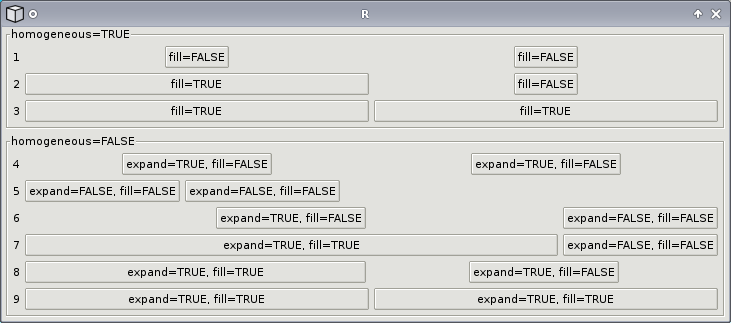
\includegraphics{packing.png}
    \caption{\label{fig:packing}A screenshot demonstrating the effect
      of packing two buttons into \class{GtkHBox} instances using the
      \method{packStart}{GtkBox} method with different combinations of
      the \argument{expand}{gtkBoxPackStart} and
      \argument{fill}{gtkBoxPackStart} settings.  The effect of the
      \argument{homogeneous}{gtkBoxPackStart} spacing setting on the
      \class{GtkHBox} is also shown.}
  \end{center}
\end{figure}

The code for some of these layouts is presented here. We begin by
creating a \class{GtkHBox} widget. We pass \code{TRUE} for the first
parameter, \argument{homogeneous}{gtkHBox}. This means that the
horizontal allocation of the box will be evenly distributed between
the children.  The second parameter directs the box to leave 5 pixels
of space between each child.  The following code constructs the
\class{GtkHBox}:
\begin{Schunk}
\begin{Sinput}
 box <- gtkHBox(TRUE, 5)
\end{Sinput}
\end{Schunk}
The equal distribution of available space is strictly enforced; the
minimum size requirement of a homogeneous box is set such that the box
always satisfies this assertion, as well as the minimum size
requirements of its children.

The \method{packStart}{GtkBox} and \method{packEnd}{GtkBox} methods pack a
widget into a box with left and right justification (top and
bottom for a \class{GtkVBox}), respectively. For this explanation, we
restrict ourselves to \method{packStart}{GtkBox}, since
\method{packEnd}{GtkBox} works the same except for the
% DTL: direction or justification?
justification. Below, we pack two buttons, \code{button\_a} and
\code{button\_b} using left justification:
\begin{Schunk}
\begin{Sinput}
 button_a <- gtkButton("Button A")
 button_b <- gtkButton("Button B")
 box$packStart(button_a, fill = FALSE)
 box$packStart(button_b, fill = FALSE)
\end{Sinput}
\end{Schunk}
%
First, \code{button\_a} is packed against the left side of the box,
and then we pack \code{button\_b} against the right side of
\code{button\_a}. This results in the first row in
Figure~\ref{fig:packing}. The space distribution is homogeneous, but
making the space available to a child does not mean that the child
will fill it. That depends on the minimum size requirement of the
child, as well as the value of the \argument{fill}{gtkBoxPackStart}
parameter passed to \method{packStart}{GtkBox}. In this case,
\argument{fill}{gtkBoxPackStart} is \code{FALSE}, so the extra space
is not filled. When a widget is packed with the
\argument{fill}{gtkBoxPackStart} parameter set to \code{TRUE}, the
widget is sized to consume the available space. This results in
rows~$2$ and $3$ in Figure~\ref{fig:packing}.

In many cases, it is desirable to give children unequal amounts of
available space, as in rows~4--9 in Figure~\ref{fig:packing}. 
% This is evident in the CRAN mirrors dialog, where the mirror list is
% given more space than the \code{Please choose a mirror} label.
To create an inhomogeneously spaced \class{GtkHBox}, we pass
\code{FALSE} as the first argument to the constructor, as in the
following code:
\begin{Schunk}
\begin{Sinput}
 box <- gtkHBox(FALSE, 5)
\end{Sinput}
\end{Schunk}

An inhomongeneous layout is freed of the restriction that all widgets
must be given the same amount of available space; it only needs to
ensure that each child has enough space to meet its minimum size
requirement. After satisfying this constraint, a box is often left
with extra space. The programmer may control the distribution of this
extra space through the \argument{expand}{gtkBoxPackStart} parameter
to \method{packStart}{GtkBox}.  When a widget is packed with
\argument{expand}{gtkBoxPackStart} set to \code{TRUE}, we will call
the widget an \emph{expanding} widget. All expanding widgets in a box
are given an equal portion of the entirety of the extra space. If no
widgets in a box are expanding, as in row~5 of
Figure~\ref{fig:packing}, the extra space is left undistributed. 

It is common to mix expanding and non-expanding widgets in the same
box.
% FIXME: do we use the mirror dialog example or another one?  For
% example, in the CRAN mirrors dialog, the box first ensures that the
% mirror list and the label above it are given enough space to satisfy
% their minimum requirement. Then, since the mirror list is expanding,
% all of the extra space is made available to it, while the label is
% left only with its minimum requirement (i.e., enough space to show
% its text).
An example is given below, where \code{button\_a} is expanding,
while \code{button\_b} is not:
\begin{Schunk}
\begin{Sinput}
 box$packStart(button_a, expand = TRUE, fill = FALSE)
 box$packStart(button_b, expand = FALSE, fill = FALSE)
\end{Sinput}
\end{Schunk}
%
The result is shown in row~6 of Figure~\ref{fig:packing}.  The figure
contains several other permutations of the
\argument{homogeneous}{gtkBoxPackStart},
\argument{expand}{gtkBoxPackStart} and
\argument{fill}{gtkBoxPackStart} settings.

\begin{figure}
  \centering
  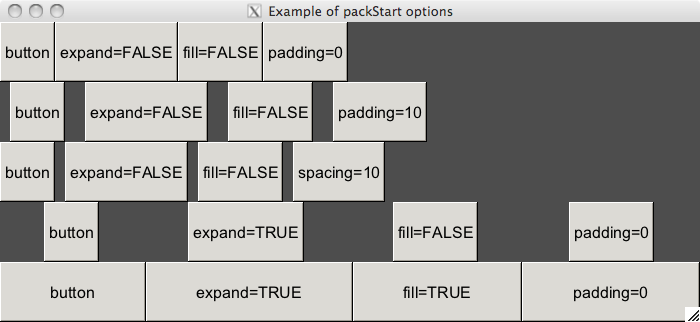
\includegraphics[width=.85\textwidth]{ex-RGtk2-pack-start}
  \caption{Examples of packing widgets into a box container. The top
    row shows no padding, whereas the 2nd and 3rd illustrate the
    difference between \code{padding} (an amount around each child)
    and \code{spacing} (an amount between each child). The last two
    rows show the effect of \code{fill} when \code{expand=TRUE}. This
    illustration follows one in orignial \GTK\/ tutorial.}
  \label{fig:RGtk2-pack-start}
\end{figure}

There are several ways to add space around widgets in a box container.
The \argument{spacing}{gtkHBox} argument for the constructors
specifies the amount of space, in pixels, between the cells. This
defaults to zero. The \code{pack} methods have a
\argument{padding}{gtkBoxPackStart} argument, also defaulting to zero,
for specifying the padding in pixels on either side of the child. It
is important to note the difference: \code{spacing} is between
children and the same for every boundary, while the \code{padding} is
specific to a particular child and occurs on either side, even on the
ends. The spacing between widgets is the sum of the \code{spacing}
value and the two \code{padding} values when the children are added.
Example~\ref{eg:RGtk2:mac-buttons} provides an example and
Figure~\ref{fig:RGtk2-pack-start} an illustration.

The \method{reorderChild}{gtkBox} method can be used
to reorder the child widgets. The new position of the child is
specified using 0-based indexing. This code will move the last child
to the second position.
\begin{Schunk}
\begin{Sinput}
 b3 <- g[[3]]
 g$reorderChild(b3, 2 - 1)               # second is 2 - 1
\end{Sinput}
\end{Schunk}

\subsection{Alignment}
\label{sec:RGtk2:layout:align}

We began this section with a simple example of a window containing a
label:
\begin{Schunk}
\begin{Sinput}
 w <- gtkWindow(show=FALSE); w$setTitle("Hello world")
 l <- gtkLabel("Hello world")
 w$add(l)
\end{Sinput}
\end{Schunk}
%
The window allocates all of its space to the label, despite the actual
text consuming a much smaller region. The size of the text is fixed,
according to the font size, so it could not be expanded. Thus, the
label decided to center the text within itself (and thus the
window). A similar problem is faced by widgets displaying images. The
image cannot be expanded without distortion. Widgets that display
objects of fixed size inherit from \class{GtkMisc}, which provides
methods and properties for tweaking how the object is aligned within
the space of the widget. For example, the \code{xalign} and
\code{yalign} properties specify how the text is aligned in our label
and take values between $0$ and $1$, with $0$ being left and
top. Their defaults are $0.5$, for centered alignment. We modify them
below to make our label left justified:
\begin{Schunk}
\begin{Sinput}
 l["xalign"] <- 0
\end{Sinput}
\end{Schunk}

Unlike a block of text or an image, a widget usually does not have a
fixed size. However, the user may wish to tweak how a widget fills
the space allocated by its container.  \GTK\/ provides the
\class{GtkAlignment} container for this purpose. For example, rather
than adjust the justification of the label text, we could have
instructed the layout not to expand but to position itself against the
left side of the window:
\begin{Schunk}
\begin{Sinput}
 w <- gtkWindow(); w$setTitle("Hello world")
 a <- gtkAlignment()
 a$set(xalign = 0, yalign = 0.5, xscale = 0, yscale = 1)
 w$add(a)
 l <- gtkLabel("Hello world")
 a$add(l)
\end{Sinput}
\end{Schunk}

\section{Buttons}
\label{sec:RGtk2:gtkButton}

The button is the very essence of a GUI. It communicates its purpose
to the user and executes a command in response to a simple click or
key press. In \GTK\/, A basic button is usually constructed using
\constructor{gtkButton}, as the following example demonstrates.

\begin{example}{Button constructors}{eg:RGtk2:button-constructors}
\begin{Schunk}
\begin{Sinput}
 w <- gtkWindow(show=FALSE)
 w$setTitle("Various buttons")
 w$setDefaultSize(400, 25)
 g <- gtkHBox(homogeneous=FALSE, spacing=5)
 w$add(g)
 b <- gtkButtonNew() 
 b$setLabel("long way")
 g$packStart(b)
 g$packStart(gtkButton(label="label only") )
 g$packStart(gtkButton(stock.id="gtk-ok") )
 g$packStart(gtkButtonNewWithMnemonic("_Mnemonic") ) # Alt-m to "click"
 w$show()
\end{Sinput}
\end{Schunk}
\end{example}

\begin{figure}
  \centering
  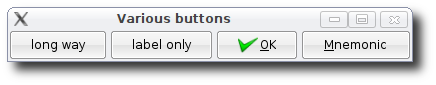
\includegraphics[width=.8\textwidth]{RGtk2-various-button}
  \caption{Various buttons}
  \label{fig:RGtk2:various-buttons}
\end{figure}

A \class{GtkButton} is simply a clickable region on the screen that is
decorated to appear as a button. \class{GtkButton} is a subclass of
\class{GtkBin}, so it will accept any widget as an indicator of its
purpose. By far the most common button decoration is a label. The
first argument of \constructor{gtkButton},
\argument{label}{gtkButton}, accepts the text for an automatically
created \class{GtkLabel}. We have seen this usage in our ``Hello
World'' example and others.

The alternative \argument{stock.id}{gtkButton} argument will use
decorations associated with the stock identifier. For example,
``gtk-ok'' would produce a button with a theme-dependent image (such
as a checkmark) and the ``Ok'' label, with the appropriate mnemonic
and translated into the current language.  The available stock
identifiers are listed by \function{gtkStockListIds}. See
\code{help(``stock-items'')} for more information.

The final button created in the example uses
\constructor{gtkButtonNewWithMnemonic} to create a button with a
mnemonic. Mnemonics are specified by prefixing the character with an
underscore.

The method \method{setRelief}{gtkButton} changes the relief style of
the button. For example, the relief can be disable so that the button
is drawn like a label.

%% signals
\paragraph{Signals}

The \signal{clicked} signal is emitted when the button is
clicked on with the mouse or when the button has focus and the
\kbd{enter} key is pressed. A callback can listen for this event to
perform a command when the button is clicked.  

\begin{example}{Callback example for
    \code{gtkButton}}{eg:RGtk2:gtkButton-callback}

\begin{Schunk}
\begin{Sinput}
 w <- gtkWindow(); b <- gtkButton("click me");
 w$add(b)
 ID <- gSignalConnect(b,"button-press-event",   # just mouse click
                      f = function(w,e,data) {
                        print(e$getButton())    # which button
                        return(FALSE)           # propogate
                      })
 ID <- gSignalConnect(b,"clicked",              # click or keyboard
                      f = function(w,...) {
                        print("clicked")
                      })
\end{Sinput}
\end{Schunk}
\end{example}

As buttons are intended to call an action immediately after being
clicked, it is customary to make them insensitive to user input when
the action is not possible. The \method{setSensitive}{gtkWidget}
method can adjust this for the button, as with other widgets.

%% Buttons initiate actions
Windows often have a default action. For example, if a window contains
a form, the default action often submits the form. If the action a
button is to initiate is the default action for the window it can be
set so that it is activated when the user presses \kbd{enter} while
the parent window has the focus. To implement this, the property
\code{can-default} must be \code{TRUE} and the widget method
\method{grabDefault}{gtkWidget} must be called. (This is not specific
to buttons, but any widget that can be activatable.)

If the action that a button initiates is to be represented elsewhere
in the GUI, say a menu bar, then a \code{GtkAction} object may be
appropriate. Action objects are covered in
Section~\ref{sec:RGtk2:UIManager}.

\begin{example}{Spacing between buttons}{eg:RGtk2:mac-buttons}
This example shows how to pack buttons into a box so that the spacing
between the similar buttons is 12 pixels, but between potentially
dangerous buttons is 24 pixels, as per the Mac human interface
guidelines.
\GTK\/ provides the constructor \constructor{gtkHButtonBox} for
holding buttons, which provides a means to apply consistent styles,
but the default styles do not allow such spacing as desired. (Had all
we wanted was to right align the buttons, then that style is certainly
supported.) As such, we will illustrate how this can be done through a
combination of \code{spacing} arguments.
We assume that our parent container, \code{g}, is a
horizontal box container.


\begin{figure}
  \centering
  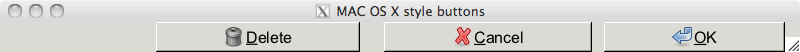
\includegraphics[width=.85\textwidth]{ex-RGtk2-mac-buttons}
  \caption{Example using stock buttons with extra spacing added between the \code{delete} and \code{cancel} buttons.}
  \label{fig:ex-RGtk2-mac-buttons}
\end{figure}

We include standard buttons, so use the stock names and icons.
\begin{Schunk}
\begin{Sinput}
 cancel <- gtkButton(stock.id="gtk-cancel")
 ok <- gtkButton(stock.id="gtk-ok")
 delete <- gtkButton(stock.id="gtk-delete")
\end{Sinput}
\end{Schunk}

We will right align our buttons, so use the parent container's
\code{PackEnd} method. The \code{ok} button has no padding, the
12-pixel gap between it and the \code{cancel} button is ensured by  the
\code{padding} argument when the \code{cancel} button is
added. Treating the \code{delete} button as potentially irreversible,
we aim to have 24 pixels of seperation between it and the
\code{cancel} button. This is given by adding 12 pixels of padding
when this button is packed in, giving 24 in total. The blank label is
there to fill out space if the parent container expands.
\begin{Schunk}
\begin{Sinput}
 g$packEnd(ok, padding=0)
 g$packEnd(cancel, padding=12)
 g$packEnd(delete, padding=12)
 g$packEnd(gtkLabel(""), expand=TRUE, fill=TRUE)
\end{Sinput}
\end{Schunk}
We make \code{ok} the default button, so have it grab the focus and
add a simple callback when the button is either clicked or the
\kbd{enter} key is pressed when the button has the focus.
\begin{Schunk}
\begin{Sinput}
 ok$grabFocus()
 QT <- gSignalConnect(ok, "clicked", function(...) print("ok"))
\end{Sinput}
\end{Schunk}






\end{example}

\section{Static Text and Images}

\subsection{Labels}
\label{sec:RGtk2:gtkLabel}

The primary purpose of a label is to communicate the role of another
widget, as we showed for the button. Labels are created by the
\constructor{gtkLabel} constructor. Its main argument is
\argument{str}{gtkLabel} to specify the button text, stored in the
\code{label} property. This text can be set with either
\method{setLabel}{gtkLabel} or \method{setText}{gtkLabel} and
retrieved with either \method{getLabel}{gtkLabel} or
\method{getText}{gtkLabel}.  The difference being the former
respects formatting marks.

\begin{example}{Label formatting}{eg:RGtk2:label-formatting}
  As all text in a \GTK\/ GUI is ultimately displayed by
  \class{GtkLabel}, there are many formatting options available.  This
  example demonstrates a sample of these~(Figure~\ref{})>
  
  \begin{figure}
    \centering
    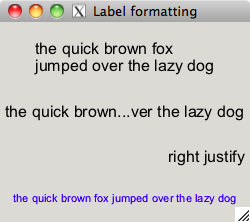
\includegraphics[width=.5\textwidth]{fig-RGtk2-labels}
    \caption{Various formatting for a label: wrapping, alignment,
      ellipsizing, PANGO markup}
    \label{fig:RGtk2:label-formatting}
  \end{figure}
  
\begin{Schunk}
\begin{Sinput}
 w <- gtkWindow(); w$setTitle("Label formatting")
 w$setSizeRequest(250,100)               # narrow
 g <- gtkVBox(spacing=2); g$setBorderWidth(5); w$add(g)
 string <- "the quick brown fox jumped over the lazy dog"
 ## wrap by setting number of characters
 basicLabel <- gtkLabel(string)
 basicLabel$setLineWrap(TRUE)
 basicLabel$setWidthChars(35)            # specify number of characters
 ## Set ellipsis to shorten long text
 ellipsized <- gtkLabel(string)
 ellipsized$setEllipsize(PangoEllipsizeMode["middle"])
 ## Right justify text lines
 ## use xalign property for aligning entire block
 rightJustified <- gtkLabel("right justify"); 
 rightJustified$setJustify(GtkJustification["right"])
 rightJustified['xalign'] <- 1
 ## PANGO markup
 pangoLabel <- gtkLabel()
 pangoLabel$setMarkup(paste("<span foreground='blue' size='x-small'>",
                            string, "</span>"))
 sapply(list(basicLabel, ellipsized, rightJustified, pangoLabel), 
        function(i) g$packStart(i,  expand = TRUE, fill = TRUE))
\end{Sinput}
\begin{Soutput}
[[1]]
NULL

[[2]]
NULL

[[3]]
NULL

[[4]]
NULL
\end{Soutput}
\begin{Sinput}
 w$showAll()
\end{Sinput}
\end{Schunk}
\end{example}

Many of the text formatting options are demonstrated in
Example~\ref{eg:RGtk2:label-formatting}. Line wrapping is enabled with
\method{setLineWrap}{gtkLabel}. Labels also support explicit line
breaks, specified with specified with ``\code{\backslashn}.'' The
\method{setWidthChars} method is a convenience for instructing the
label to request enough space to show a specified number of
characters in a line.  When space is at a premium, long labels can be
ellipsized, i.e., have their text truncated and appended with an
ellipsis, ``...''.  By default this is turned off; to enable, call
\method{setEllipsize}{gtkLabel}.  The property \code{justify}, with
values taken from \code{GtkJustification}, controls the alignment of
multiple lines within a label. To align the entire block of text
within the space allocated to the label, modify the \code{xalign}
property, as described in Section~\ref{sec:RGtk2:layout:align}.

\GTK\/ allows markup of text elements using the Pango text attribute
markup language, an XML-based format that resembles basic HTML. The
method \method{setMarkup}{gtkLabel} accepts text in the format. Text
is marked using tags to indicate the style. Some convenient tags are
\code{<b>} for bold, \code{<i>} for italics, \code{<ul>} for
underline, and \code{<tt>} for monospace text. More complicated markup
involves the \code{<span>} tag markup, such as \code{<span
  color='red'>some text</span>}. The text can may need to be escaped
first, so that designated entities replace reserved characters.

Although mostly meant for static text display, \class{GtkLabel} has
some interactive features. If the \code{selectable} property is set to
\code{TRUE}, the text can be selected and copied into the clipboard.
Labels can hold mnemonics for other widgets; this is useful for
navigating forms. The mnemonic is specified at construction time with
\code{gtkLabelNewWithMnemonic}. The
\method{setMnemonicWidget}{gtkLabel} method identifies the widget to
which the mnemonic refers.


%% signals
\paragraph{Signals}
Unlike buttons, labels do not emit any specific signals, as they are
intended to hold static text. Although a label is a \class{GtkWidget},
it does not receive any system events. A work-around is to place the
label within an instance of \class{GtkEventBox}. This creates a
non-visible parent window for the label that listens to the windowing
system. Example~\ref{eg:RGtk2:editable-label} will illustrate the use
of an event box.  Alternatively, if a clickable label is desired, one
could use an instance of \code{gtkButton} with its \code{relief}
property assigned to \code{GtkReliefStyle['none']}.

%% ML: Better to just update RGtk2 and talk about the 2.18 support for
%% links in label markup. Link buttons are pretty limited in comparison.

% \subsection{Link Buttons}
% \label{sec:link-buttons}

% A link button is a special label which shows an underlined link, such
% as is done by a web browser (newer versions of \GTK\/ allow the label
% of a button to contain HTML links). The \code{uri} is specified to the
% \constructor{gtkLinkButton} constructor with an optional
% \argument{label}{gtkLinkButton} argument. If none is specified, the
% \code{uri} is used to provide the value. This \code{uri} is stored in
% the \code{uri} property and the label in the \code{label} value. These
% may be adjusted later.

% As the link button inherits from the \class{gtkButton} class, the
% \code{clicked} signal is emitted when a user clicks a mouse on the link.

% \begin{example}{Basic link button usage}{eg:RGtk2:link-button}
% <<LinkButton>>=
% w <- gtkWindow()
% g <- gtkVBox(); w$add(g)
% lb <- gtkLinkButton(uri="http://www.r-project.org")
% lb1<- gtkLinkButton(uri="http://www.r-project.org", label="R Home")
% g$packStart(lb)
% g$packStart(lb1)

% f <- function(w,...) browseURL(w['uri'])

% ID <- gSignalConnect(lb,  "clicked", f = f)
% ID <- gSignalConnect(lb1, "clicked", f = f)
% @ 
% \end{example}

\subsection{Statusbars}
\label{sec:RGtk2:statusbars}

In \GTK, a statusbar is constructed through the
\constructor{gtkStatusbar} function. Statusbars must be placed at the
bottom of a top-level window by the programmer. In \GTK, a statusbar
keeps various stacks of messages for display. One adds a message to
display for given stack through the \method{Push}{gtkStatusbar} method
by specifying first an integer value for \code{context.id} and a
message. To pop the top message on a stack and display the next, the
method \method{Pop}{gtkStatusbar} method is available.

\subsection{Images}
\label{sec:RGtk2:images}

It is said that a picture can be worth a thousand words, and images
are often a more space efficient alternative to
labels. \class{GtkImage} is the widget that displays images. The
constructor \constructor{gtkImage} supports creating images from
various in-memory image representations, files, and other sources.  We
only discuss loading an image from a file. Images can be loaded after
construction, as well. For example, the \method{setFromFile}{gtkImage}
method loads an image from a file.

The image widget, like the label widget, does not have a parent
\class{GdkWindow}, which means it does not receive window events. As
with the label widget, the image widget can be placed inside a
\constructor{gtkEventBox} container if one wishes to connect to such
events.



\begin{example}{Using a pixmap to present graphs}{ex:RGtk2:pixbuf}

  This example shows how to use a \constructor{GtkImage} object to
  embed a graphic within \pkg{RGtk2}, using the
  \pkg{cairoDevice} package. The basic idea is to draw onto an
  off-screen pixmap using \pkg{cairoDevice} and
  then to construct a \class{GtkImage} from the pixmap. 

  We begin by creating a window of a certain size.
\begin{Schunk}
\begin{Sinput}
 w <- gtkWindow(show=FALSE); w$setTitle("Graphic window");
 w$setSizeRequest(400,400)
 g <- gtkHBox(); w$add(g)
 w$showAll()
\end{Sinput}
\end{Schunk}


The size of the image is retrieved from the size allocated to the box
\code{g}. This allows the window to be resized prior to drawing the
graphic. Unlike an interactive device, after drawing, this graphic
does not resize itself when the window resizes.

\begin{Schunk}
\begin{Sinput}
 theSize <- g$getAllocation()
 width <- theSize$width; height <- theSize$height
\end{Sinput}
\end{Schunk}

Now we create a \class{GdkPixmap} of the correct dimensions and
initialize an R graphics device that targets the pixmap. We then draw
a simple histogram using base R graphics.
\begin{Schunk}
\begin{Sinput}
 require(cairoDevice)
 pixmap <- gdkPixmap(drawable = NULL, width = width, height = height,
                     depth = 24)
 asCairoDevice(pixmap)
\end{Sinput}
\begin{Soutput}
[1] TRUE
\end{Soutput}
\begin{Sinput}
 hist(rnorm(100))
\end{Sinput}
\end{Schunk}

The final step is to create the \class{GtkImage} widget to display the
pixmap: 
\begin{Schunk}
\begin{Sinput}
 image <- gtkImage(pixmap = pixmap)
 g$packStart(image, expand=TRUE, fill = TRUE)
\end{Sinput}
\end{Schunk}

\end{example}


\subsection{Stock icons}
\label{sec:RGtk2:stock-icons}

In \GTK\/, standard icons, like the one on the ``OK'' button, can be
customized by themes. This is implemented by a database that maps a
\textit{stock} identifier to an icon image. The stock identifier
corresponds to a commonly performed type of action, such as the ``OK''
response or the ``Save'' operation. There is no hard-coded set of
stock identifiers, however \GTK\/ provides a default set for the most
common operations. These identifiers are all prefixed with
``gtk-''. Users may register new types of stock icons.
%% ML: I believe there is an example of this in the RGtk2 demos

As mentioned previously, the full list of stock icons are returned in
a list by \function{gtkStockListIds}. The first $4$ are:
\begin{Schunk}
\begin{Sinput}
 head(unlist(gtkStockListIds()), n=4)   
\end{Sinput}
\begin{Soutput}
[1] "gtk-zoom-out" "gtk-zoom-in"  "gtk-zoom-fit" "gtk-zoom-100"
\end{Soutput}
\end{Schunk}

The use of stock identifiers over specific images is encouraged, as it
allows an application to be customized through themes. The
\constructor{gtkButton} and \constructor{gtkImage} constructors accept
a stock identifer passed as \code{stock.id} argument, and the icons in
toolbars and menus are most conveniently specified by stock
identifier. 

% ML: Sorry, but I am not sure if this illustrates an important concept


% In the example below, we use the method \method{renderIcon}{gtkWidget} to
% return a pixbuf containing the icon that can be used with the
% constructor \constructor{gtkImageNewFromPixbuf} to display the
% icon. Here the stock id and size are specified to the
% \method{renderIcon}{gtkWidget} method.

% \begin{example}{\constructor{gtkButtonNewFromStock} -- the hard way}{ex:RGtk2:stock-icon}
% \SweaveInput{ex-RGtk2-button-new-stock-hardway}
% \end{example}

% ML: Could this example be in the book, but marked as optional or advanced?

%% Only for the package
%% Adding icons to stock
\begin{example}{Adding to the stock icons}{ex:RGtk2:add-stock-icons}
This example shows, without much explanation the steps to add images
to the list of stock icons. To generate some sample icons, we use
those provided by objects in the \pkg{ggplot2} package.




First we create the icons using the fact that the objects have a function \code{icon} to draw an image.
\begin{Schunk}
\begin{Sinput}
 require(ggplot2)
 iconNames <- c("GeomBar","GeomHistogram")   # 2 of many ggplot functions
 icon.size <- 16
 pixbufs <- sapply(iconNames, function(name) {
   pixmap <- gdkPixmap(drawable = NULL, width = icon.size, height = icon.size,
                       depth = 24)
   asCairoDevice(pixmap)
   val <- try(get(name))
   grid.newpage()
   try(grid.draw(val$icon()), silent=TRUE)
   dev.off()
   gdkPixbufGetFromDrawable(NULL, pixmap, NULL, 0, 0, 0, 0, -1 -1)
 })
\end{Sinput}
\end{Schunk}
The following function works through the steps to add a new icon. The
basic ideas are sketched out in the API for \code{GtkIconSet}.
\begin{Schunk}
\begin{Sinput}
 addToStockIcons <- function(pixbufs, stock.prefix="new") {
   iconfactory <- gtkIconFactory()
   
   items <- lapply(names(pixbufs), function(iconName) {
     ## each icon has its own icon set, which is registered with icon factory
     iconset <- gtkIconSetNewFromPixbuf(pixbufs[[iconName]])
     stockName <- paste(stock.prefix, "-", iconName, sep="")
     iconfactory$add(stockName, iconset)
     
     ## create stock item for icon
     as.GtkStockItem(list(stock_id = stockName, label = iconName))
   })
   ## register our factory of icons
   iconfactory$addDefault()
   ## officially register the stock items
   gtkStockAdd(items)
 }
\end{Sinput}
\end{Schunk}
We call this function and then check that the values are added:
\begin{Schunk}
\begin{Sinput}
 addToStockIcons(pixbufs)
 nms <- gtkStockListIds()
 unlist(nms[grep("^new", nms)])
\end{Sinput}
\end{Schunk}

\end{example}



%% Alertpanel application
\begin{example}{An alert panel}{eg:RGtk2:alert-panel}

\begin{figure}
  \centering
  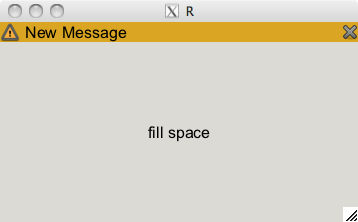
\includegraphics[width=.45\textwidth]{ex-RGtk2-alert-panel}
  \caption{The alert panel showing a message.}
  \label{fig:RGtk2-alert-panel}
\end{figure}

This example puts together images, buttons, labels and box containers
to create an alert panel, or information bar. This is an area that
seems to drop down from the menu bar to give users feedback about an
action that is less disruptive than a modal dialog. A similar widget
is used in the Firefox browser with its popup blocker. Although, as of version
2.18, a similar feature is available in \GTK\/ through the
\code{GtkInfoBar} widget, this example is given, as it shows how
several useful things in \GTK\/ can be combined to customize the user
experience.

This constructor for the widget specifies some properties and returns
an environment to store these properties, as our function calls will
need to update these properties and have be persistent.
\begin{Schunk}
\begin{Sinput}
 newAlertPanel <- function(wrap=35,
                           icon="gtk-dialog-warning",
                           message="",
                           panel.color="goldenrod",
                           evb=NULL,
                           image=NULL,
                           label=NULL # info
                     ) {
   x <- c("wrap","icon","message","panel.color","evb","image","label")
   e <- new.env()
   sapply(x, function(i) assign(i, envir=e, get(i)))
   return(e)
 }
\end{Sinput}
\end{Schunk}

An alert panel needs just a few methods: one to create the widget, one
to show the widget and one to hide the widget. We create a function
\code{getAlertPanelBlock} to return a component that can be added to a
container. An event box is used so that we can color the background,
as this isn't possible for a box container due to its lack of a gdk
window.  To this event box we add a box container that will hold an
icon indicating this is an alert, a label for the message, and another
icon to indicate to the user how to close the alert. Since we wish to
receive mouse clicks on close icon, we place this inside another event
box. To this, we bind a callback to the \signal{button-press-event} signal.
\begin{Schunk}
\begin{Sinput}
 getAlertPanelBlock <- function(obj) {
 
   obj$evb <- gtkEventBox(show=FALSE)
   obj$evb$ModifyBg(state="normal",color=obj$panel.color)
 
   g <- gtkHBox(homogeneous=FALSE, spacing=5)
   obj$evb$add(g)
 
   obj$image <- gtkImageNewFromStock(obj$icon, size="button")
   obj$image['yalign'] <- .5
   g$packStart(obj$image, expand=FALSE)
 
   obj$label <- gtkLabel(obj$message)
   obj$label['xalign'] <- 0; obj$label['yalign'] <- .5
   obj$label$setLineWrap(TRUE)
   obj$label$setWidthChars(obj$wrap)
   g$packStart(obj$label, expand=TRUE, fill=TRUE)
 
   xbutton <- gtkEventBox()
   xbutton$modifyBg(state="normal", color=obj$panel.color) 
   xbutton$add(gtkImageNewFromStock("gtk-close", size="menu"))
   g$packEnd(xbutton, expand=FALSE, fill=FALSE)
   xbuttonCallback <- function(data, widget,...) {
     hideAlertPanel(data)
     return(FALSE)
   }
 
   ## close on button press and event box click
   sapply(list(xbutton, obj$evb), function(i) {
     gSignalConnect(i, "button-press-event",
                    f=xbuttonCallback,
                    data=obj, user.data.first=TRUE)
     })
   return(obj$evb)
 }
\end{Sinput}
\end{Schunk}

The \code{showAlertPanel} function updates the message and then calls
the \method{Show}{gtkWidget} method of the event box.

\begin{Schunk}
\begin{Sinput}
 showAlertPanel <- function(obj) {
   obj$label$setText(obj$message)
   obj$evb$show()
 }
\end{Sinput}
\end{Schunk}

Our \code{hideAlertPanel} function simply calls the \method{hide}{gtkWidget}
method the event box.
\begin{Schunk}
\begin{Sinput}
 hideAlertPanel <- function(obj) obj$evb$hide()
\end{Sinput}
\end{Schunk}

To test it out, we create a simple GUI
\begin{Schunk}
\begin{Sinput}
 w <- gtkWindow()
 g <- gtkVBox(); w$add(g)
 ap <- newAlertPanel()
 g$packStart(getAlertPanelBlock(ap), expand=FALSE)
 g$packStart(gtkLabel("fill space"), expand=TRUE, fill=TRUE)
 ap$message <- "New Message"             # add message
 showAlertPanel(ap)
\end{Sinput}
\end{Schunk}

To improve this, one could also add a time to close the panel after some delay. The
\function{gTimeoutAdd} function is used to specify a function to call
periodically until the function returns \code{FALSE}.

\end{example}

\section{Input Controls}

\subsection{Text entry}
\label{sec:RGtk2:gtkEntry}

The widgets explained thus far are largely static. For example, \GTK\/
does not yet support editable labels. Text editing is handled by other
widgets that are rendered in the familiar depressed box form. We will
discuss complex multi-line text editing in
Section~\ref{sec:RGtk2:textviews}. For entering a single line of text,
the \class{GtkEntry} widget is appropriate.  It is constructed by
\function{gtkEntry}. An argument \argument{max}{gtkEntry} specifies
the maximum number of characters if positive, but this calls a
deprecated function. Instead, call the method
\method{setMaxLength}{gtkEntry} after construction.

The \code{text} property stores the text. This can be set with the
method \method{setText}{gtkEntry} and retrieved with
\method{getText}{gtkEntry}. Editing text programmatically relies on
the \class{GtkEditable} interface, which \class{GtkEntry}
implements. The method \method{insertText}{GtkEditable} inserts text.
Its argument \argument{new.text}{gtkEditableInsertText} contains the
text and \argument{position}{gtkEditableInsertText} specifies the
position of the text to be added. The return value is a list with the
component \code{position} indicating the position \textit{after} the
new text. The \method{deleteText}{GtkEditable} method deletes
text. This takes two integers indicating the start and finish location
of the text to delete.

\begin{example}{Insert and Delete text}{eg:RGtk2:insert-delete-text}
The example will show how to add then delete text.  
\begin{Schunk}
\begin{Sinput}
 e <- gtkEntry()
 e$setText("Where did that guy go?")
 add.pos <- regexpr("guy", e['text']) - 1 # before "guy"
 ret <- e$insertText("@$#%! ", position = add.pos)
 e$getText()                             # or e['text']
\end{Sinput}
\begin{Soutput}
[1] "Where did that @$#%! guy go?"
\end{Soutput}
\begin{Sinput}
 e$deleteText(start = add.pos, end= ret$position)
 e$getText()
\end{Sinput}
\begin{Soutput}
[1] "Where did that guy go?"
\end{Soutput}
\end{Schunk}
\end{example}

%% signals
The \class{GtkEditable} interface supports three signals:
\signal{changed} when text is changed, \signal{delete-text} for delete
events, and \signal{insert-text} for insert events. It is possible to
prevent the insertion or deletion of text by connecting to the
corresponding signal and stopping the signal propagation with
\function{gSignalStopEmission}. 

\class{GtkEntry} defines a number of its own signals, including the
\signal{activate} signal, which is emitted when the \kbd{enter} key is
pressed.

%% skipped
%% ML: I agree; kind of a hack
% \begin{example}{Editable label}{eg:RGtk2:editable-label}
%   \SweaveInput{ex-RGtk2-editable-label}
% \end{example}


\subsection{Check button}
\label{sec:RGtk2:gtkCheckbox}
%% TODO: example in this section

Very often, the action performed by a button simply changes the value
of a state variable in the application. \GTK\/ defines several types
of buttons that explicitly manage and display the value of a state
variable. The simplest type of state variable is binary (boolean) and is
usually proxied by a \class{GtkCheckButton}. 

A \class{GtkCheckButton} is constructed by
\function{gtkCheckButton}. The optional argument
\argument{label}{gtkCheckButton} places a label next to the
button. The alternative constructor
\constructor{gtkCheckButtonewWithMnemonic} gives the label a mnemonic.

As with any \class{GtkButton}, the \code{label} property stores the
label.  The state of the binary variable is represented by the
\code{active} property. It can be set or retrieved with the methods
\method{setActive}{gtkToggleButton} and
\method{getActive}{gtkToggleButton}.

When the state is changed the \signal{toggle} signal is emitted. The
callback should check the \code{active} property to determine if the
button has been enabled or disabled.

An alternative to \class{GtkCheckButton} is the lesser used
\class{GtkToggleButton}, which is actually the parent class of
\class{GtkCheckButton}. A toggle button is drawn as an ordinary
button. It remains depressed while the state variable is \code{TRUE},
instead of relying on a checkbox to communicate the binary value.

\subsection{Radio button group}
\label{sec:RGtk2:gtkRadioButton}

\GTK\/ provides two button types for discrete state variables that
accept more than two possible values: combo boxes, discussed in the
next section, and radio buttons. The \function{gtkRadioButton}
constructor creates an instance of \class{GtkRadioButton}, an
extension of \class{GtkCheckButton}. Each radio button belongs to a
group.  There is no explicit group object; rather, the buttons are
chained together as a linked list. By default, a newly constructed
button is added to its own group. If \argument{group}{gtkRadioButton}
is a list of radio buttons, the newly created button is added to the
group. The constructor returns a single radio button widget.

%% active
Like other types derived from \class{GtkToggleButton}, each radio
button in the group has an \code{active} property.  Only one button in
the group can have \code{active} set to \code{TRUE} at a time. To
determine which button is active, each button needs to be queried
individually. Setting \code{active} to \code{TRUE} activates the
corresponding button and ensures that the other buttons are disabled.

\begin{example}{Radio group construction}{eg:RGtk2:radio-buttons}
Creating a new radio button group with the basic
\constructor{gtkRadioButton} constructor follows this pattern:
\begin{Schunk}
\begin{Sinput}
 vals <- c("two.sided", "less", "greater")
 radiogp <- list()                                 # list for group
 radiogp[[vals[1]]] <- gtkRadioButton(label=vals[1]) # group = NULL
 for(i in vals[-1]) 
   radiogp[[i]] <- gtkRadioButton(radiogp, label=i)  # group is a list
\end{Sinput}
\end{Schunk}
Each button needs to be managed. Here we illustrate a simple GUI doing so.
\begin{Schunk}
\begin{Sinput}
 w <- gtkWindow(); w$setTitle("Radio group example")
 g <- gtkVBox(FALSE, 5); w$add(g)
 sapply(radiogp, gtkBoxPackStart, object = g)
\end{Sinput}
\begin{Soutput}
$two.sided
NULL

$less
NULL

$greater
NULL
\end{Soutput}
\end{Schunk}
We can set and query which button is active, as follows:
\begin{Schunk}
\begin{Sinput}
 g[[3]]$setActive(TRUE)           
 sapply(radiogp, `[`, "active") 
\end{Sinput}
\begin{Soutput}
two.sided      less   greater 
    FALSE     FALSE      TRUE 
\end{Soutput}
\end{Schunk}
Here is how we might register a callback for the \code{toggled} signal.
\begin{Schunk}
\begin{Sinput}
 sapply(radiogp, gSignalConnect, "toggled",     # attach each to "toggled"
        f = function(w, data) {
          if(w$getActive()) # set before callback
            cat("clicked", w$getLabel(),"\n")
        })
\end{Sinput}
\begin{Soutput}
two.sided.toggled      less.toggled   greater.toggled 
              135               136               137 
\end{Soutput}
\end{Schunk}
\end{example}

The \method{getGroup}{gtkRadioButton} method returns a list containing
the radio buttons in the same group. However, it is in the reverse
order of construction (newest first). This results from an internal
optimization that prepends, rather than appends, the buttons to a
linked list.
% ML: wow! they can't reverse the list?

As a convenience, there are constructor functions ending with
\code{FromWidget} that determine the group from a radio button
belonging to the group. As we will see in our second example, this
allows for a more natural \function{sapply} idiom that avoids the need
to allocate a list and populate it in a \code{for} loop.

\begin{example}{Radio group using \code{getGroup}}{eg:gtk:radio-group-get-group}
  In this example below, we illustrate two things: using the
  \constructor{gtkRadioButtonNewWithLabelFromWidget} function to add new
  buttons to the group and the \method{GetGroup}{gtkRadioButton}
  method to reference the buttons. The \function{rev} function is used
  to pack the widgets, to get them to display first to last.
\begin{Schunk}
\begin{Sinput}
 radiogp <- gtkRadioButton(label=vals[1])
 sapply(vals[-1], gtkRadioButtonNewWithLabelFromWidget, group = radiogp)
\end{Sinput}
\begin{Soutput}
$less
<pointer: 0x4076238>
attr(,"interfaces")
[1] "AtkImplementorIface" "GtkBuildable"       
attr(,"class")
 [1] "GtkRadioButton"    "GtkCheckButton"    "GtkToggleButton"  
 [4] "GtkButton"         "GtkBin"            "GtkContainer"     
 [7] "GtkWidget"         "GtkObject"         "GInitiallyUnowned"
[10] "GObject"           "RGtkObject"       

$greater
<pointer: 0x40762b0>
attr(,"interfaces")
[1] "AtkImplementorIface" "GtkBuildable"       
attr(,"class")
 [1] "GtkRadioButton"    "GtkCheckButton"    "GtkToggleButton"  
 [4] "GtkButton"         "GtkBin"            "GtkContainer"     
 [7] "GtkWidget"         "GtkObject"         "GInitiallyUnowned"
[10] "GObject"           "RGtkObject"       
\end{Soutput}
\begin{Sinput}
 w <- gtkWindow(); 
 w['title'] <- "Radio group example"
 g <- gtkVBox(); w$add(g)
 sapply(rev(radiogp$getGroup()), gtkBoxPackStart, object = g)
\end{Sinput}
\begin{Soutput}
[[1]]
NULL

[[2]]
NULL

[[3]]
NULL
\end{Soutput}
\end{Schunk}
\end{example}

\subsection{Combo boxes}
\label{sec:RGtk2:basic-combobox}

The combo box is a more space efficient alternative to radio buttons
and is better suited for when there are a large number of options. A
basic, text-only \class{GtkComboBox} is constructed by
\constructor{gtkComboBoxNewText}. Later we will discuss more
complicated combo boxes, where an underlying data model is
manipulated.
% Unlike
% others, as of writing, this widget must have its
% \method{Show}{gtkWidget} method called to be mapped.

For the basic combo box, items may be added in a few different ways.
The methods \method{appendText}{gtkComboBox} and
\method{prependText}{gtkComboBox} add a text item to the end or
beginning, respectively.  A text item is inserted at an arbitrary
position in the list with the \method{insertText}{gtkComboBox}.

The currently selected value is specified by index with the method
\method{setActive}{gtkComboBox} and returned by
\method{getActive}{gtkComboBox}. The index, as usual, is $0$-based,
and in this case, a value of $-1$ indicates that no value is selected.
The \method{getActiveText}{gtkComboBox} method can be used to retrieve
the text shown by the basic combo box.

Although combo boxes are much more space efficient than radio buttons,
it can be difficult to use a combo box when there are a large number
of selections. The \method{setWrapWidth}{gtkComboBox} method specifies
the preferred number of columns for displaying the items.


%% signal
The main signal to connect to is \signal{changed} which is emitted
when the active item is changed either by the user or the programmer
through the \code{getActive} method.

\begin{example}{Combo box}{eg:RGtk2:simple-combo-box}
A simple combo box may be produced as follows:
\begin{Schunk}
\begin{Sinput}
 vals <- c("two.sided", "less", "greater")
 cb <- gtkComboBoxNewText()
 sapply(vals, gtkComboBoxAppendText, object = cb)
\end{Sinput}
\begin{Soutput}
$two.sided
NULL

$less
NULL

$greater
NULL
\end{Soutput}
\begin{Sinput}
 cb$setActive(0)                         # first one
 gSignalConnect(cb, "changed",
                f = function(w, ...) {
                  i <- w$getActive() + 1 # shift index
                  if(i == 0) 
                    cat("No value selected\n")
                  else
                    cat("Value is", w$getActiveText(), "\n")
                })
\end{Sinput}
\begin{Soutput}
changed 
    166 
attr(,"class")
[1] "CallbackID"
\end{Soutput}
\begin{Sinput}
 w <- gtkWindow(show=FALSE)
 w['title'] <- "Combobox example"
 w$add(cb)
 w$show()
\end{Sinput}
\end{Schunk}
\end{example}

\subsection{Sliders}
\label{sec:RGtk2:sliders}

The slider widget and spin button widget allow selection from a
regularly spaced, semi-continuous list of values.

The slider widget is called \class{GtkScale} and may be oriented
either horizontally or vertically. This depends on the constructor:
\constructor{gtkHScale} or \constructor{gtkVScale}.  The user must
specify the minimum, maximum and step values for the scale.  This set
of values is formally represented by the \class{GtkAdjustment}
structure. Ordinarily, it is not necessary to construct a
\class{GtkAdjustment} explicitly. Instead, the constructors accept the
the numeric arguments \argument{min}{gtkHScale}, \argument{max}{gtkHScale},
and \argument{step}{gtkHScale}.

The underlying \class{GtkAdjustment} serves as the data model for the
slider. Multiple sliders can be synchronized by attaching to the same
adjustment object.

The methods \method{getValue}{gtkRange} and
\method{setValue}{gtkRange} can be used to get and set the value of
the widget. Values are clamped to the bounds defined by the
adjustment.

%% properties
A few properties define the appearance of the slider widget.  The
\code{digits} property controls the number of digits after the decimal
point.  The property \code{draw-value} toggles the drawing of the
selected value near the slider. Finally, \code{value-pos}
specifies where this value will be drawn using values from
\code{GtkPositionType}. The default is \code{top}.

%% value-changed
Callbacks can be assigned to the \code{value-changed} signal, which is
emitted when the slider is moved.

\begin{example}{A slider controlling histogram bin selection}{ex:RGtk2:sliders}
  A simple mechanism to make a graph interactive is to redraw the graph
  whenever a slider, controlling a plot parameter, is changed. The
  following shows how this can be achieved.
\begin{Schunk}
\begin{Sinput}
 library(lattice)
 w <- gtkWindow(); w$setTitle("Histogram bin selection")
 slider <- gtkHScale(min = 1, max = 100, step = 1)
 slider$setValue(10)                        # initial val.
 slider['value-pos'] <- "bottom"
 w$add(slider)
 drawHistogram <- function(val) print(histogram(x, nint = val))
 gSignalConnect(slider, "value-changed",
                f = function(w, ...) {
                  val <- w$getValue()
                  drawHistogram(val)
                })
\end{Sinput}
\begin{Soutput}
value-changed 
          174 
attr(,"class")
[1] "CallbackID"
\end{Soutput}
\begin{Sinput}
 x <- rnorm(100)                         # the data
 drawHistogram(slider$getValue())                    # initial graphic
\end{Sinput}
\end{Schunk}
\end{example}

\subsection{Spin buttons}
\label{sec:RGtk2:spinboxes}

The spin button widget is very similar to the slider widget,
conceptually and in terms of the \GTK\/ API. Spin buttons are
constructed with \constructor{gtkSpinButton}. As with sliders, this
constructor requires specifying adjustment values, either as a
\class{GtkAdjustment} or individually. 

As with sliders, the methods \method{getValue}{gtkSpinButton} and
\method{setValue}{gtkSpinButton} get and set the widgets
value. The property \code{snap-to-ticks} can be set to \code{TRUE} to
force the new value to belong to the sequence of values in the
adjustment. The \code{wrap} property indicates if the sequence will
``wrap'' around at the bounds.

The \code{value-changed} signal is emitted when the spin button is
changed, as with sliders.

\begin{example}{A range widget}{ex:RGtk2-range-widget}
This example shows how to make a range widget that combines both the
slider and spinbutton to choose a single number. Such a widget is
popular, as the slider is better at large changes and the spin button
better at finer changes. In \GTK\/ we use the same
\class{GtkAdjustment} model, so changes to one widget propogate
without effort to the other.


Were this written as a function, an \R\/ user might expect the
arguments to match those of \code{seq}:
\begin{Schunk}
\begin{Sinput}
 from <- 0; to <- 100; by <- 1
\end{Sinput}
\end{Schunk}

The slider is drawn without a value, as the value is already displayed
by the spin button. The call to \constructor{gtkHScale} implicitly
creates an adjustment for the slider. The spin button is created with
the same adjustment.
\begin{Schunk}
\begin{Sinput}
 slider <- gtkHScale(min=from, max=to, step=by)
 slider['draw-value'] <- FALSE
 adjustment <- slider$getAdjustment()
 spinbutton <- gtkSpinButton(adjustment = adjustment)
\end{Sinput}
\end{Schunk}
%
Our layout places the two widgets in a horizontal box container with
the slider set to expand into the available space, but not the
spinbutton.
\begin{Schunk}
\begin{Sinput}
 g <- gtkHBox()
 g$packStart(slider, expand=TRUE, fill=TRUE, padding=5)
 g$packStart(spinbutton, expand=FALSE, padding=5)
\end{Sinput}
\end{Schunk}


\end{example}

\section{Containers}
\label{sec:containers}

In Section~\ref{RGtk2:layout}, we presented \class{GtkBox} and
\class{GtkAlignment}, the two most useful layout containers in
\GTK. This section introduces some other important containers. These
include the merely decorative \class{GtkFrame}; the interactive
\class{GtkExpander}, \class{GtkPaned} and \class{GtkNotebook}; and the
grid-style layout container \class{GtkTable}. All of these widgets are
derived from \class{GtkContainer}, and so share methods like
\method{add}{GtkContainer}, which adds a child.

\subsection{Framed containers}
\label{sec:RGtk2:gtkFrame}

The \constructor{gtkFrame} function constructs a container that draws
a decorative, labeled frame around its single child. This is useful
for visually segregating a set of conceptually related widgets from
the rest of the GUI.  The optional \argument{label}{gtkFrame} argument
specifies the label text, stored in the \code{label} property. The
\method{setLabelAlign}{gtkFrame} aligns the label relative to the
frame.  Frames have a decorative shadow whose type, a value of
\code{GtkShadowType}, is stored in the \code{shadow-type} property.

\subsection{Expandable containers}
\label{sec:RGtk2:gtkExpander}

The \class{GtkExpander} widget provides a button that hides and shows
a single child upon demand. This is often an effective mechanism for
managing screen space. Expandable containers are constructed by
\function{gtkExpander}. Use \function{gtkExpanderNewWithMnemonic} if a
mnemonic is desired. The label text can be passed to the constructor
or set later with the \method{setLabel}{gtkExpander} method. The
\code{expanded} property, which can be accessed with
\method{getExpanded}{gtkExpander} and
\method{setExpanded}{gtkExpander}, represents the visible state of the
widget.  When the \code{expanded} property changes, the
\signal{activate} signal is emitted.


\subsection{Notebooks}
\label{sec:RGtk2:gtkNotebook}

The \constructor{gtkNotebook} constructor creates a notebook
container, a widget that displays an array of buttons resembling
notebook tabs. Each tab corresponds to a widget, and when a tab is
selected, its widget is made visible, while the others are hidden. If
\class{GtkExpander} is like a check button, \class{GtkNotebook} is
like a radio button group. 

The current page number is stored in the \code{page} property.  The
total number of pages is returned by \method{getNPages}{gtkNotebook}.
The default position of the notebook tabs is on the top, ordered from
left to right. The property \code{tab-pos} represents the tab position
with a value from \code{GtkPositionType}: \qcode{left}, \qcode{right},
\qcode{top}, or \qcode{bottom}.

%% adding pages
\paragraph{Adding pages to a notebook}
New pages can be added to the notebook with the
\method{InsertPage}{gtkNotebook} method, which takes the widget
associated with the page, the $0$-based insertion position (defaults
to last), as well as
a widget, such as a \class{GtkLabel} instance, not a string, to label
the tab. This allows for more complicated tabs, such as a box
container with a label and close icon. The
\method{setTabLabelText}{gtkNotebook} method is a convenience for
setting a label as text.  To use this method, the child widget is
needed, which can be retrieved with the \method{[[}{GObject}
%% ]]
%% 
method or the \method{getNthPage}{gtkNotebook} method. Both are a
shortcut around retrieving all of the children as a list through
\method{getChildren}{gtkContainer}. 

%% page motions: reordered, deleted
\paragraph{Manipulating pages}

Methods that manipulate pages operate on the page number. To map from
the child widget to the page number, use the method
\method{pageNum}{gtkNotebook}.   A given page can be raised with the
\method{setCurrentPage}{gtkNotebook} method.  Incremental movements
are possible through the methods \method{nextPage}{gtkNotebook} and
\method{prevPage}{gtkNotebook}.

Pages can be reordered using the \method{reorderChild}{gtkNotebook},
although it is usually desirable to allow the user to reorder
pages. The \method{setTabReorderable}{GtkNotebook} enables drag and
drop reordering for a specific tab. It is also possible for the user
to drag and drop pages between notebooks. Pages can be deleted using
the method \method{removePage}{gtkNotebook}.

\paragraph{Managing Many Pages}

By default, a notebook will request enough space to display all of its
tabs. If there are many tabs, space may be wasted. \class{GtkNotebook}
solves this with the scrolling idiom. If the
property \code{scrollable} is set to \code{TRUE}, arrows will be added
to allow the user to scroll through the tabs. In this case, the tabs
may become difficult to navigate. Setting the \code{enable-popup}
property to \code{TRUE} enables a right-click popup menu listing all
of the tabs for direct navigation.

\paragraph{Signals}

The notebook widget emits signals when pages are toggled, added,
removed, and reordered. The most useful is likely to be
\signal{switch-page}, which is emitted when the current page is
changed.

\begin{example}{Adding a page with a close button}{eg:RGtk2-notebook-close-icon}
  A familiar element of notebooks in many web browsers is a tab close
  button. The following defines a new method
  \method{insertPageWithCloseButton}{gtkNotebook} that will use the
  themeable stock close icon.  The callback passes both the notebook
  and the page through the \code{data} argument, so that the proper
  page can be deleted.

\begin{Schunk}
\begin{Sinput}
 gtkNotebookInsertPageWithCloseButton <- 
   function(object, child, label.text="", position=-1) {
     label <- gtkHBox()
     label$packStart(gtkLabel(label.text))
     icon <- gtkImage(pixbuf = object$renderIcon("gtk-close", "button"))
     closeButton <- gtkButton()
     closeButton$setImage(icon)
     label$packEnd(closeButton)
     ID <- gSignalConnect(b,"clicked",
                          function(userData, b, ...) {
                            nb <- userData$nb 
                            page <- userData$page
                            nb$removePage(nb$pageNum(page))
                          },
                          data = list(nb=object, page=child),
                          user.data.first=TRUE)
     object$insertPage(child, label, position)
   }
\end{Sinput}
\end{Schunk}

We now show a simple usage of a notebook.
\begin{Schunk}
\begin{Sinput}
 w <- gtkWindow()
 nb <- gtkNotebook(); w$add(nb)
 nb$setScrollable(TRUE)
 nb$insertPageWithCloseButton(gtkButton("hello"), 
                              label.text="page 1")
\end{Sinput}
\begin{Soutput}
[1] 0
\end{Soutput}
\begin{Sinput}
 nb$insertPageWithCloseButton(gtkButton("world"), 
                              label.text="page 2")
\end{Sinput}
\begin{Soutput}
[1] 1
\end{Soutput}
\end{Schunk}
  
\end{example}


\subsection{Scrollable windows}
\label{sec:RGtk2:scroll-windows}

The \class{GtkExpander} and \class{GtkNotebook} widgets support
efficient use of screen real estate. However, when a widget is always
too large to fit in a GUI, partial display is necessary. A
\class{GtkScrolledWindow} supports this by providing scrollbars for
the user to adjust the visible region of a single child. The range, step
and position of \class{GtkScrollbar} are controlled by an instance of
\class{GtkAdjustment}, just as with the slider and spin button.

The constructor \constructor{gtkScrolledWindow} creates a
\class{GtkScrolledWindow} instance. By default, the horizontal and
vertical adjustments are automatically determined, although they may
be overridden by the programmer.

The widget in a scrolled window must know how to display only a part
of itself, i.e., it must be scrollable. Some widgets, including
\class{GtkTreeView} and \class{GtkTextView}, have native scrolling
support. Other widgets must be embedded within the proxy
\class{GtkViewport}. The \class{GtkScrolledWindow} convenience method
\method{addWithViewport}{GtkScrolledWindow} allows the programmer to
skip the \class{GtkViewport} step.

The properties \code{hscrollbar-policy} and \code{vscrollbar-policy}
determine when the scrollbars are drawn. By default, they are always
drawn. The \qcode{automatic} value from the \code{GtkPolicyType}
enumeration draws the scrollbars only if needed, i.e, the
child widget requests more space than can be allocated. The
\method{setPolicy}{gtkScrolledWindow} method allows both to be set at
once, as in the following example.

\begin{example}{Scrolled window example}{eg:RGtk2:scrolled-window}
This example shows how to display a long list of values with scrolled
windows. The tree view widget can also do this, but here we can very
easily customize the display of each value. In the example, we simply
locates where a label is placed.

%% ML: Don't like this example too much: scrolling over labels does
%% not seem realistic. The most natural example in my mind is a
%% GtkDrawingArea displaying R graphics. A plot can essentially be
%% zoomed and panned with GtkViewport.


\begin{Schunk}
\begin{Sinput}
 g <- gtkVBox(spacing=0)
 sapply(state.name, function(i) {
   l <- gtkLabel(i)
   l['xalign'] <- 0; l['xpad'] <- 10
   g$packStart(l, expand=TRUE, fill=TRUE)
 })
\end{Sinput}
\begin{Soutput}
$Alabama
NULL

$Alaska
NULL

$Arizona
NULL

$Arkansas
NULL

$California
NULL

$Colorado
NULL

$Connecticut
NULL

$Delaware
NULL

$Florida
NULL

$Georgia
NULL

$Hawaii
NULL

$Idaho
NULL

$Illinois
NULL

$Indiana
NULL

$Iowa
NULL

$Kansas
NULL

$Kentucky
NULL

$Louisiana
NULL

$Maine
NULL

$Maryland
NULL

$Massachusetts
NULL

$Michigan
NULL

$Minnesota
NULL

$Mississippi
NULL

$Missouri
NULL

$Montana
NULL

$Nebraska
NULL

$Nevada
NULL

$`New Hampshire`
NULL

$`New Jersey`
NULL

$`New Mexico`
NULL

$`New York`
NULL

$`North Carolina`
NULL

$`North Dakota`
NULL

$Ohio
NULL

$Oklahoma
NULL

$Oregon
NULL

$Pennsylvania
NULL

$`Rhode Island`
NULL

$`South Carolina`
NULL

$`South Dakota`
NULL

$Tennessee
NULL

$Texas
NULL

$Utah
NULL

$Vermont
NULL

$Virginia
NULL

$Washington
NULL

$`West Virginia`
NULL

$Wisconsin
NULL

$Wyoming
NULL
\end{Soutput}
\end{Schunk}

The scrolled window has just two basic steps in its construction. Here
we specify never using a scrolled window for the vertical display.
\begin{Schunk}
\begin{Sinput}
 sw <- gtkScrolledWindow()
 sw$setPolicy("never","automatic")
 sw$addWithViewport(g)                   # just "Add" for text, tree, ...
\end{Sinput}
\end{Schunk}

\begin{Schunk}
\begin{Sinput}
 w <- gtkWindow(show=FALSE)
 w$setTitle("Scrolled window example")
 w$setSizeRequest(-1, 300)
 w$add(sw)
 w$show()
\end{Sinput}
\end{Schunk}
\end{example}

\subsection{Divided containers}
\label{sec:RGtk2:gtkPanedWindow}

The \constructor{gtkHPaned} and \constructor{gtkVPaned} create
containers that contain two widgets, arranged horizontally or
vertically and separated by a handle.  The user may adjust the
position of the handle to apportion the allocation between the
widgets.
% An example is presented in Example \ref{eg:RGtk2:using-tree-content}. 

The two children may be added two different ways. The methods
\method{pack1}{gtkPaned} and \method{pack2}{gtkPaned} have arguments
\argument{resize}{gtkPanedPack1}, whether the child expands with the
parent, and \argument{shrink}{gtkPanedPack1}, whether the widget is
allowed to shrink. The methods \method{add1}{gtkPaned} and
\method{add2}{gtkPaned} add children such that both are allowed to
shrink and only the second widget expands.  After children are added,
they can be referenced from the container through the
\method{getChild1}{gtkPaned} and \method{getChild2}{gtkPaned} methods.

The screen position of the handle can be set with the
\method{setPosition}{gtkPaned} method.  The properties
\code{min-position} and \code{max-position} can be used to convert a
percentage into a screen position. The \signal{move-handle} signal is
emitted when the gutter position is changed.




\subsection{Tabular layout}
\label{sec:RGtk2:gtkTable}

The \constructor{gtkTable} constructor produces a container for laying
out objects in a tabular format. The container sets aside cells in a
grid, and a child widget may occupy one or more cells. The
\argument{homogeneous}{gtkTable} argument can be used to make all
cells homogeneous in size. Otherwise, each column and row can have a
different size. At the time of construction, the number rows and
columns for the table many be specified with the
\argument{rows}{gtkTable} and \argument{columns}{gtkTable}
arguments. After construction, the \method{Resize}{gtkTable} method
can be used to resize these values.

%% adding children
Child widgets are added to this container through the
\method{attach}{gtkTable} method. Its first argument,
\argument{child}{gtkTableAttach}, is the child widget. This widget can
span more than one cell. The arguments
\argument{left.attach}{gtkTableAttach} and
\argument{right.attach}{gtkTableAttach} specify the horizontal bounds
of the child in terms of its left column and right column,
respectively. Analogously, \argument{top.attach}{gtkTableAttach} and
\argument{bottom.attach}{gtkTableAttach} define the vertical bounds.
By default, the widgets will expand into and fill the available space,
much as if \argument{expand}{gtkBoxPackStart} and
\argument{fill}{gtkBoxPackStart} were passed as \code{TRUE} to
\method{packStart}{GtkBox} (see
Section~\ref{sec:RGtk2:layout:box}). There is no padding between
children by default. Both the resizing behavior and padding may be
overridden by specifying additional arguments to
\method{attach}{GtkTable}.

The child properties \code{xalign} and \code{yalign} specify the
alignment of child widgets within their allocated space. These behave
as with \class{GtkAlignment}.

%% JV: this doesn't add enough it seems
% \begin{example}{Layout of calculator buttons}{eg-RGtk2-calculator-buttons}
%   \SweaveInput{ex-RGtk2-calculator-buttons.Rnw}
% \end{example}


\begin{example}{Dialog layout}{ex-RGtk2-dialog-layout}
This example shows how to layout some controls for a dialog with some
attention paid to how the widgets are aligned and how they respond to
resizing of the window.

\begin{figure}
  \centering
  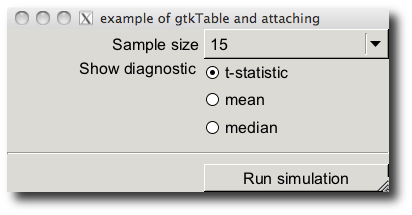
\includegraphics[width=.5\textwidth]{ex-RGtk2-dialog-layout}
  \caption{A basic dialog using a \code{gtkTable} container for layout.}
  \label{fig:RGtk2-dialog-layout}
\end{figure}


Our basic GUI is a table with 4 rows and 2 columns.
\begin{Schunk}
\begin{Sinput}
 w <- gtkWindow(show=FALSE)
 w$setTitle("example of gtkTable and attaching")
 tbl <- gtkTable(rows=4, columns=2, homogeneous=FALSE)
 w$add(tbl)
\end{Sinput}
\end{Schunk}

We define our widgets first then deal with their layout.
\begin{Schunk}
\begin{Sinput}
 l1 <- gtkLabel("Sample size")
 w1 <- gtkComboBoxNewText()
 QT <- sapply(c(5, 10, 15, 30), function(i) w1$appendText(i))
 l2 <- gtkLabel("Show diagnostic ")
 w2 <- gtkVBox()
 rb <- list()
 rb[["t"]] <- gtkRadioButton(label="t-statistic")
 for(i in c("mean","median")) rb[[i]] <- gtkRadioButton(rb, label=i)
 QT <- sapply(rb, function(i) w2$packStart(i))
 w3 <- gtkButton("Run simulation")
\end{Sinput}
\end{Schunk}

The basic \code{AttachDeafults} method will cause the widgets to
expand when resized, which we want to control here. As such we use
\code{Attach}. To get the control's label to center align yet still
have some breathing room we set its
\code{xalign} and  \code{xpad} properties.
For the combobox we avoid using \qcode{expand} as otherwise it resizes
to fill the space allocated to the cell in the \code{y} direction.
\begin{Schunk}
\begin{Sinput}
 tbl$attach(l1, left.attach=0,1, top.attach=0,1, yoptions="fill")
 l1["xalign"] <- 1; l1["xpad"] <- 5
 tbl$attach(w1, left.attach=1,2, top.attach=0,1, xoptions="fill", yoptions="fill")
\end{Sinput}
\end{Schunk}

We use \qcode{expand} here to attach the radio group, so that it
expands to fill the space. The label has its \code{yalign} proporty
set, so that it stays at the top of the cell, not the middle.
\begin{Schunk}
\begin{Sinput}
 tbl$attach(l2, left.attach=0,1, top.attach=1,2, yoptions="fill")
 l2["xalign"] <- 1; l2['yalign'] <- 0; l2["xpad"] <- 4
 tbl$attach(w2, left.attach=1,2, top.attach=1,2, xoptions=c("expand", "fill"))
\end{Sinput}
\end{Schunk}
A separator with a bit of padding provides a visual distinction
between the controls and the button to initiate an action.
\begin{Schunk}
\begin{Sinput}
 tbl$attach(gtkHSeparator(),left.attach=0,2, top.attach=2,3, ypadding=10, yoptions="fill")
 tbl$attach(w3, left.attach=1,2, top.attach=3,4, xoptions="fill", yoptions="fill")
\end{Sinput}
\end{Schunk}
Finally, we use the \code{ShowAll} method so that it propogates to the combobox.
\begin{Schunk}
\begin{Sinput}
 w$showAll()                             # propogate to combo
\end{Sinput}
\end{Schunk}
\end{example}


%% JV: this is in need of rewriting
\section{Drag and drop}
\label{sec:RGtk2:dnd}

%% ------------ Drag and Drop

\GTK\/ has mechanisms to provide drag and drop facilities for
widgets. To setup drag and drop actions requires setting a widget to
be a source for a drag request, and setting a widget to be a target
for a drop action, and assigning callbacks to responsd to certain
signals.  Only widgets which can receive signals will work for drag
and drop, so to drag or drop on a label, say, an event box must be
used. 

We illustrate how to set up the dragging of a text value from one
widget to another. Much more complicated examples are possible, but we
do not pursue it here.

When a drag and drop is initiated, different types of data may be
transferred. \GTK\/ allows the user to specify a target type. Below,
we define target types for text and pixmap objects. These
give numeric IDs for lookup purposes.
\begin{Schunk}
\begin{Sinput}
 TARGET.TYPE.TEXT   <- 80                 
 TARGET.TYPE.PIXMAP <- 81                  
\end{Sinput}
\end{Schunk}
We use of these to make different types of objects that can be dragged.
\begin{Schunk}
\begin{Sinput}
 widgetTargetTypes <- list(
 ## target -- string representing the drag type. MIME type used.
 ## flag delimiting drag scope. 0 -- no limit
 ## info -- application assigned value to identify
 text = gtkTargetEntry("text/plain", 0, TARGET.TYPE.TEXT),
 pixmap = gtkTargetEntry("image/x-pixmap", 0, TARGET.TYPE.PIXMAP)
 )
\end{Sinput}
\end{Schunk}

\paragraph{A drag source}
A widget that can have a value dragged from it is a drag source. It is
specifide by calling
\function{gtkDragSourceSet}. This function has arguments
\argument{object}{gtkDragSourceSet} for the widget we are making a
source, \argument{start.button.mask}{gtkDragSourceSet}  to specify
which mouse buttons can initiate the drag,
\argument{targets}{gtkDragSourceSet} to specify the target type, and
\argument{actions}{gtkDragSourceSet} to indicate which of the
\code{GdkDragAction} types is in effect, for instance \code{copy} or
\code{move}. 

When a widget is a drag source, it sends the data being dragged in
response to the \signal{drag-data-get} signal using a callback. The
signature of this callback is important, although we only use the
\code{selection} argument, as this is assigned the text that will be the
data passed to the target widget. (Text, as we are passing text
information.)

\begin{Schunk}
\begin{Sinput}
 w <- gtkWindow(); w['title'] <- "Drag Source"
 dragSourceWidget <-  gtkButton("Drag me")
 w$add(dragSourceWidget)
 QT <- gtkDragSourceSet(dragSourceWidget,
                  start.button.mask=c("button1-mask", "button3-mask"),
                  targets=widgetTargetTypes[["text"]],
                  actions="copy") ## can also be any of GdkDragAction
 ID <- 
   gSignalConnect(dragSourceWidget, "drag-data-get", 
                  f=function(widget, context, 
                    selection, targetType, eventTime) {
                    ## customize this to set the text
                    selection$setText(str="some value") 
                  })
\end{Sinput}
\end{Schunk}

\paragraph{Drop target}
To make a widget a drop target, we call \function{gtkDragDestSet} on
the object with the argument \argument{flags}{gtkDragDestSet} for
specifying the actions \GTK\/ will perform when the widget is dropped
on. We use the value \qcode{all} for \qcode{motion},
\qcode{highlight}, and \qcode{drop}. The
\argument{targets}{gtkDragDestSet} argument matches the type of data
being allowed, in this case text. Finally, the value of
\argument{action}{gtkDragDestSet} specifies what \code{GdkDragAction}
should be sent back to the drop source widget. If the action was
\qcode{move} then the source widget emits the \code{drag-data-delete}
signal, so that a callback can be defined to handle the deletion of
the data.

 
\begin{Schunk}
\begin{Sinput}
 w <- gtkWindow(); w['title'] <- "Drop Target"
 dropTargetWidget <- gtkButton("Drop here")
 w$add(dropTargetWidget)
 QT <- gtkDragDestSet(dropTargetWidget,
                      flags="all", 
                      targets=widgetTargetTypes[["text"]],
                      actions="copy"
                      )
\end{Sinput}
\end{Schunk}

When data is dropped, the widget emits the
\code{drag-data-received}. The data is passed through the
\code{selection} argument. The \code{context} argument is a
\code{gdkDragContext}, containing information about the drag
event. The \code{x} and \code{y} arguments are integer valued and pass
in the position in the widget where the drop occurred. In the example
below, we see that text data is passed to this function in \code{raw}
format, so it is converted with \function{rawToChar}.

\begin{Schunk}
\begin{Sinput}
 ID <- 
   gSignalConnect(dropTargetWidget, "drag-data-received", 
                  f=function(dropTargetWidget, 
                    context, x, y, 
                    selection, targetType, eventTime) {
                    dropdata <- selection$getText()
                    if(class(dropdata)[1] == "raw")
                      val <- paste(rawToChar(dropdata), sep="")
                    else
                      val <- paste(dropdata, sep="")
                    print(val) ## some action
                  })
\end{Sinput}
\end{Schunk}

%% JV: This could be expanded -- motion is not covered, as is done with
%% tcltk, but I don't think it is needed without a compelling use case.

\section{Graphics}

% Describe GdkDrawable, GdkPixbuf, Cairo, GtkDrawingArea

\subsection{The cairoDevice package}
\label{sec:cairodevice-package}

The package \pkg{cairoDevice} is an R graphics device based on the
Cairo graphics library.  It is cross-platform and supports
alpha-blending and antialiasing. Through its support for the
\function{getGraphicsEvent} function, it is currently the most
interactive cross-platform graphics device.  

\pkg{RGtk2} and \pkg{cairoDevice} are integrated through the
\function{asCairoDevice} function. If a \class{GtkDrawingArea},
\class{GdkDrawable}, \class{Cairo} context, or \class{GtkPrintContext}
is passed to \function{asCairoDevice}, an R graphics device will be
initialized that targets its drawing to the object. For simply
displaying graphics in a GUI, the \class{GtkDrawingArea} is the best
choice. 
% TODO: put GtkDrawingArea example here
For more complex use cases, such as compositing a layer above
or below the R graphic, one should pass an off-screen
\class{GdkDrawable}, like a \class{GdkPixmap}, or a \class{Cairo}
context. The off-screen drawing can then be composited with other
images when displayed. Finally, passing a \class{GtkPrintContext} to
\function{asCairoDevice} allows printing R graphics through the \GTK\/
printing dialogs.


%% FIXME: could rename to Widgets for Viewing Data
%% Then could add cairoDevice, introduction to GDK/Cairo
%% Visualization is pretty important
\chapter{RGtk2: Widgets Using Models}
\label{sec:RGtk2:widgets-with-models}

%% Possible outline:
%% - Displaying tabular data (GtkTreeView)
%%   - Loading data frame
%%   - Displaying data frame
%%   - Accessing GtkTreeModel (to set up selection, and hierarchical data)
%%   - Selection (an important concept, but common to hierarchical, below)
%%   - Sorting/filtering
%%   - Cell renderer details
%% - Displaying hierarchical data (GtkTreeView)
%%   - Loading hierarchical data
%%   - Displaying data as a tree
%% - Model-based combo boxes
%% - Text entry completion
%% - Icon views (currently omitted, probably OK)
%% - Text views

%% TODO: we need a unified example in the main text that spans loading
%% a data frame to sorting a model, at least.

Many widgets in \GTK\/ use the model, view, controller (MVC)
paradigm. For most, like the button, the MVC pattern is implicit;
however, widgets that primarily display data explicitly incorporate
the MVC pattern into their design. The data model is factored out as a
separate object, while the widget plays the role of the view and
controller. The MVC approach adds a layer of complexity but
facilitates the display of the dynamic data in multiple, coordinated
views.

\section{Display of tabular data}
\label{sec:RGtk2:tabular-heirarchical-data}

Widgets that display lists, tables and trees are all based on the same
basic data model, \class{GtkTreeModel}. Although its name suggests a
hierarchical structure, \class{GtkTreeModel} is also tabular. We first
describe the display of an \R\/ data frame in a list or table
view. The display of hierarchical data, as well as further details of
the \class{GtkTreeModel} framework, are treated subsequently.

\subsection{Loading a data frame}
\label{sec:tabular-stores-tree}

As an interface, \class{GtkTreeModel} may be implemented in any number
of ways. \GTK\/ provides simple in-memory implementations for
hierarchical and non-hierarchical data. For improved speed,
convenience and familiarity, \pkg{RGtk2} includes a custom
\class{GtkTreeModel} implementation called class{RGtkDataFrame}, which
is based on an \R\/ data frame. For non-hierarchical data, this is
usually the model of choice, so we discuss it first.

\R\/ uses data frames to hold tabular data, where each column is of a
certain class, and each row is related to some observational
unit. This fits the structure of \class{GtkTreeModel} when there is no
hierarchy. As such it is natural to have a means to map a data frame
into a store for a tree view. \class{RGtkDataFrame} implements
\class{GtkTreeModel} to perform this role and is constructed with the
\constructor{rGtkDataFrame} function. Populating a
\class{RGtkDataFrame} is much faster than a \GTK\/ model, because the
data is taken directly from the data frame, without any copying or
need to add each row individually in a slow \R\/ loop. The constructor
takes a data frame as an argument. The column classes are important,
so even if this data frame is empty, the user should specify the
desired column classes upon construction.

An object of class \class{RGtkDataFrame} supports the familiar S3
methods \method{[}{RGtkDataFrame}, \method{[\ASSIGN}{RGtkDataFrame},
\method{dim}{RGtkDataFrame}, and
\method{as.data.frame}{RGtkDataFrame}. The \code{[$<$-} method does
not have quite the same functionality as it does for a data
frame. Columns can not be removed by assigning values to \code{NULL},
and column types should not be changed. These limitations are inherit
in the design of \GTK: columns may not be removed from
\class{GtkTreeModel}, and views expect the data type to remain the
same.

\begin{example}{Defining and manipulating a \class{RGtkDataFrame}}{eg-RGtk2-manipulate-rGtkDataframe}
  The basic data frame methods are similar.
\begin{Schunk}
\begin{Sinput}
 data(Cars93, package="MASS")            # mix of classes
 model <- rGtkDataFrame(Cars93)
 model[1, 4] <- 12
 model[1, 4]                              # get value
\end{Sinput}
\begin{Soutput}
[1] 12
\end{Soutput}
\end{Schunk}

Factors are treated differently from character values, as is done with
data frames, so assignment to a factor must be from one of the
possible levels.

\end{example}

The data frame combination functions \Rfunction{rbind} and
\Rfunction{cbind} are unsupported, as they would create a new data
model, rather than modify the model in place. Thus, one should add
rows with \method{appendRows}{rGtkDataFrame} and add columns with
\method{appendColumns}{rGtkDataFrame} (or sub-assignment, 
\method{[\ASSIGN}{RGtkDataFrame}).

The \method{setFrame}{rGktDataFrame} method replaces the underlying
data frame.
\begin{Schunk}
\begin{Sinput}
 model$setFrame(Cars93[1:5, 1:5])
\end{Sinput}
\begin{Soutput}
NULL
\end{Soutput}
\end{Schunk}
%
Replacing the data frame is the only way to remove rows, as this is
not possible with conventional data frame sub-assignment
interface. Removing columns or changing their types remains
impossible. The new data frame cannot contain more columns and rows
than the current one. If the new data frame has more rows or columns,
then the appropriate \code{append} method should be used first.

\subsection{Displaying data as a list or table}
\label{sec:RGtk2:mvc:GtkTreeView}

%% intro
\class{GtkTreeView} is the primary view of \class{GtkTreeModel}.  It
serves as the list, table and tree widget in \GTK. A tree view is
essentially a container of columns, where every column has the same
number of rows. If the view has a single column, it is essentially a
list. If there are multiple columns, it is a table. If the rows are
nested, it is a tree table, where every node has values on the same
columns.

%% constructor
A tree view is constructed by \constructor{gtkTreeView}. 
\begin{Schunk}
\begin{Sinput}
 view <- gtkTreeView(model)
\end{Sinput}
\end{Schunk}
Usually, as in the above, the model is passed to the
constructor. Otherwise, the model may be accessed with
\method{setModel}{gtkTreeView} and \method{getModel}{gtkTreeView}.

A newly created tree view displays zero columns, regardless of the
number of columns in the model. Each column, an instance of
\class{GtkTreeViewColumn}, must be constructed, inserted into the view and
instructed to render content based on one or more columns in the data
model:
\begin{Schunk}
\begin{Sinput}
 vc <- gtkTreeViewColumn()
 vc$setTitle("Manufacturer")
 cr <- gtkCellRendererText()
 vc$packStart(cr)
 vc$addAttribute(cr, "text", 0)
 view$insertColumn(vc, 0)
\end{Sinput}
\begin{Soutput}
[1] 1
\end{Soutput}
\end{Schunk}
%
A column with
the title ``Manufacturer'' is inserted at the first, $0$-based,
position. For displaying a simple data frame, we only need to render
text. Each row in a column consists of one or more cells, managed in a
layout. The number of cells and how each cell is rendered is uniform
down a column. As an implementation of \class{GtkCellLayout},
\class{GtkTreeViewColumn} delegates the responsibility of rendering to
one or more \class{GtkCellRenderer} objects. The cell renderers are
packed into the column, which behaves much like a box
container. Rendering of text cells is the role of
\class{GtkCellRendererText}; we create an instance with
\constructor{gtkCellRendererText}. There are several properties that
control how the text is rendered. A so-called \textit{attribute} links
a model column to a renderer property. The most important property is
\code{text}, the text itself. In the example, we bind the \code{text}
property to the first ($0$-indexed) column in the model.

\class{GtkTreeView} provides the \method{insertColumnWithAttributes}
convenience method to perform all of these steps with a single
call. We invoke it to add a second column in our view:
\begin{Schunk}
\begin{Sinput}
 view$insertColumnWithAttributes(position = -1, title = "Model", 
                                 cell = gtkCellRendererText(), text = 1)
\end{Sinput}
\begin{Soutput}
[1] 2
\end{Soutput}
\end{Schunk}
% 
The $-1$ passed as the first argument indicates that the column should
be appended. Next, we specify the column title, a cell renderer, and
an attribute that links the \code{text} renderer property to the
second column in the model. In general, any number of attributes may
be defined after the third argument.  We will use the above idiom in
all of the following examples, as it is much more concise than
performing each step separately.

To display the entire Cars93 data frame, we insert a view column for
every column in the data frame. Here, we reconstruct the view, inserting
a view column for every column in the data frame, i.e., the model.
\begin{Schunk}
\begin{Sinput}
 view <- gtkTreeView(model)
 f <- function(...) view$insertColumnWithAttributes(...)
 mapply(f,  -1, colnames(model), 
        list(gtkCellRendererText()), text = seq_len(ncol(model)) - 1)
\end{Sinput}
\begin{Soutput}
[1] 1 2 3 4 5
\end{Soutput}
\end{Schunk}
%
Although it was relatively easy to create a \class{GtkTreeModel} for
the data frame using \class{RGtkDataFrame}, the complexity of
\class{GtkTreeView} complicates the task of displaying the data frame
in a simple, textual table. When this is all that is necessary, one
might consider \function{gdataframe} from \pkg{gWidgets}. For those
who wish to render text in each row differently (e.g., in a different
color) or fill cells with images, check boxes, progress bars and the
like, direct use of the \class{GtkTreeView} API is required.

\paragraph{Manipulating view columns}

The \Rclass{GtkTreeView} widget is essentially a collection of
columns. Columns are added to the tree view with the methods
\method{insertColumn}{gtkTreeView} or, as shown above,
\method{insertColumnWithAttributes}{gtkTreeView}.  A column can be
moved with the \method{moveColumnAfter}{gtkTreeView} method, and
removed with the \method{removeColumn}{gtkTreeView} method. The
\method{getColumns}{gtkTreeView} method returns a list containing all
of the tree view columns.

There are several properties for controlling the behavior and
dimensions of a \class{GtkTreeViewColumn} instance. The property
\qcode{resizable} determines wheter the user can resize a column, by
dragging with the mouse. The size properties \qcode{width},
\qcode{min-width}, and \qcode{fixed-width} control the size. The
visibility of the column can be adjusted through the
\method{setVisible}{gtkTreeViewColumn} method.

\paragraph{Additional Features}

Tree views have several special features, including sorting,
incremental search and drag-n-drop reordering. Sorting is discussed in
Section~\ref{sec:RGtk2:mvc:proxies}. To turn on searching,
\code{enable-search} should be \code{TRUE} (the default) and the
\code{search-column} property should be set to the column to be
searched. The tree view will popup a search box when the user types
\kbd{control-f}. To designate an arbitrary text entry widget as the
search box, call \method{setSearchEntry}{GtkTreeView}. The entry can
be placed anywhere in the GUI. Columns are always reorderable by drag
and drop. Reordering rows through drag-and-drop is enabled by the
\code{reorderable} property.

\paragraph{Aesthetic properties}

\Rclass{GtkTreeView} is capable of rendering some visual guides. The
\code{rules-hint}, if \code{TRUE}, will instruct the theme to draw
rows in alternating colors. To show grid lines, set
\code{enable-grid-lines} to \code{TRUE}.

\subsection{Accessing \class{GtkTreeModel}}
\label{sec:RGtk2:mvc:iterators}

Although \class{RGtkDataFrame} provides a familiar interface for
manipulating the data in a \class{GtkTreeModel}, it is often necessary
to directly interact with the \GTK\/ API, such a when using another
type of data model or interpreting user selections. There are two
primary ways to index into the rows of a tree model: paths and
iterators.

To index directly into an arbitrary row, a \class{GtkTreePath} is
appropriate. For a list, a tree path is essentially the row number,
$0$-based; for a tree it is a sequence of integers referring to the
offspring index at each level. The sequence of integers may be
expressed as either a numeric/integer vector or a string, using
\constructor{gtkTreePathNewFromIndices} or
\constructor{gtkTreePathNewFromString}, respectively. For a flat list
model, there is only one integer in the sequence:
\begin{Schunk}
\begin{Sinput}
 secondRow <- gtkTreePathNewFromIndices(2)
\end{Sinput}
\end{Schunk}
Referring to a row in a hierarchy is slightly more complex:
\begin{Schunk}
\begin{Sinput}
 abcPath <- gtkTreePathNewFromIndices(c(1, 3, 2))
 abcPath <- gtkTreePathNewFromString("1:3:2")
\end{Sinput}
\end{Schunk}
In the above, both paths refer to the second child of the third child
of the first top-level node. To recover the integer or string
representation of the path, use \method{getIndices}{GtkTreePath} or
\method{toString}{GtkTreePath}, respectively.

%% iters

The second means of row indexing is through an iterator,
\class{GtkTreeIter}, which is better suited for traversing a model.
While a tree path is an intuitive, transparent row index, an iterator,
by contrast, is an opaque index that is efficiently incremented. It is
probably most common for a model to be accessed in an iterative
manner, so all of the data accessor methods for \class{GtkTreeModel}
expect \class{GtkTreeIter}, not \class{GtkTreePath}. The \GTK\/
designers imagined that the typical user would obtain an iterator for
the first row and to visit each row in sequence:
\begin{Schunk}
\begin{Sinput}
 iter <- model$getIterFirst()
 manufacturer <- character()
 flag <- iter$retval
 while(flag) {
   manufacturer <- c(manufacturer, model$get(iter$iter, 0)[[1]])
   flag <- model$iterNext(iter$iter)
 }
\end{Sinput}
\end{Schunk}
%
In the above, we recover the manufacturer column from the Cars93 data
frame. Whenever a \class{GtkTreeIter} is returned by a
\class{GtkTreeModel}, the return value in \R\/ is a list of two
components: \code{retval}, a logical indicating whether the iterator
is valid, and \code{iter}, the pointer to the underlying C data
structure. The call to \method{get}{GtkTreeModel} also returns a list,
with an element for each column index passed as an argument. The
method \method{iterNext}{gtkTreeStore} updates the passed iterator in
place, i.e., by reference, to point to the next row. Thus, no new
iterator is returned. This is unfamiliar behavior in \R. Instead, the
method returns a logical value indicating whether the iterator is
still valid, i.e. \code{FALSE} is returned if no next row exists.

It is clear that the above usage is designed for languages like C,
where multiple return values are conveniently passed by reference
parameters. The iterator design also prevents the use of the apply
functions, which are generally preferred over the \code{while} loop
for reasons of performance and clarity. An improvement would be to
obtain the number of children, generate the sequence of row indices
and access the row for each index:
\begin{Schunk}
\begin{Sinput}
 nrows <- model$iterNChildren(NULL)
 manufacturer <- sapply(seq(nrows), function(i) {
   iter <- model$iterNthChild(NULL, i)
   model$get(iter$iter, 0)[[1]]
 })
\end{Sinput}
\end{Schunk}
%
Here we use \code{NULL} to refer to the virtual root node that sits
above the rows in our table. Unfortunately, this usage too is
unintuitive and slow, so the benefits of \class{RGtkDataFrame} should
be obvious.

One can convert between the two representations. The method
\method{getIter}{GtkTreeModel} on \class{GtkTreeModel} returns an
iterator for a path. A shortcut from the string representation of the
path to an iterator is \method{getIterFromString}{GtkTreeModel}. The
path pointed to by an iterator is returned by
\method{getPath}{GtkTreeModel}.

One might note that \class{GtkTreeIter} is created and managed by the
model, while \class{GtkTreePath} is model independent. It is not
possible to use iterators across models or even across modifications
to a model. After a model changes, an iterator is invalid. A tree path
may still point to a valid row, though it will not in general be the
same row from before the change. To refer to the same row across tree
model changes, use a \class{GtkTreeRowReference}, not discussed
further.

\subsection{Selection}
%% selection: none, single browse multiple, getSelected

There are multiple modes of user interaction with a tree view: if the
cells are not editable, then selection is the primary mode.  A single
click selects the value, and a double click is often used to initiate
an action. If the cells are editable, then a double click or a click
on an already selected row will initiate editing of the
content. Editing of cell values is a complex topic and is handled by
derivatives of \class{GtkCellRenderer}, see
Section~\ref{sec:RGtk2:cellrenderers}. Here, we limit our discussion
to selection of rows.

\GTK\/ provides the class \Rclass{GtkTreeSelection} to manage row
selection. Every tree view has a single instance of
\Rclass{GtkTreeSelection}, returned by the
\method{getSelection}{gtkTreeView} method.

The usage of the selection object depends on the selection mode, i.e.,
whether multiple rows may be selected. The mode is configured with the
\method{setMode}{gtkTreeSelection} method, with values from
\code{GtkSelectionMode}, including \qcode{multiple} for allowing more
than one row to be selected and \qcode{single} for limiting selections
to a single row, or none.

When only a single selection is possible, the method
\method{getSelected}{gtkTreeSelection} returns the selected row as
list, with components \code{retval} to indicate success, \code{model}
pointing to the tree model and \code{iter} representing an iterator to
the selected row in the model.

\begin{Schunk}
\begin{Sinput}
 model <- rGtkDataFrame(mtcars)
 view <- gtkTreeView(model)
 selection <- view$getSelection()
 selection$setMode("single")
\end{Sinput}
\end{Schunk}

\begin{Schunk}
\begin{Soutput}
[1] 1
\end{Soutput}
\end{Schunk}
%
If this tree view is shown and a selection made, this code will
return the value in the first column:
\begin{Schunk}
\begin{Sinput}
 selection$selectPath(gtkTreePathNewFromIndices(3)) # set 
 # 
 curSel <- selection$getSelected()       # retrieve selection
 with(curSel, model$getValue(iter, 0)$value) # model, iter
\end{Sinput}
\begin{Soutput}
[1] 21.4
\end{Soutput}
\end{Schunk}

When multiple selection is permitted, then the method
\method{getSelectedRows}{gtkTreeSelection} returns a list with
componets \code{model} pointing to the model, and \code{retval}, a list
of tree paths. 

For example, we can change the selection mode as follows.
\begin{Schunk}
\begin{Sinput}
 selection$setMode("multiple")
\end{Sinput}
\end{Schunk}

This code will print the selected values in the first column (we have
selected the first three rows):
\begin{Schunk}
\begin{Sinput}
 curSel <- selection$getSelectedRows()
 if(length(curSel$retval)) {
   rows <- sapply(curSel$retval, gtkTreePathGetIndices) + 1L
   curSel$model[rows, 1]
 }
\end{Sinput}
\begin{Soutput}
[1] 21.0 22.8 21.4
\end{Soutput}
\end{Schunk}

To respond to a selection, connect to the \signal{changed} signal on
\Rclass{GtkTreeSelection}. The signal itself does not contain any
selection information; the selection object should be queried instead.

%% double click
When a row is not editable, then the double-click event or a keyboard
command triggers the \signal{row-activated} signal for the tree
view. The callback has arguments \code{tree.view} pointing to the
widget that emits the signal, \code{path} storing a tree path of the
selected row, and \code{column} containing the tree view column. The
column number is not returned. If that is of interest, it can be
passed in via the user data argument, or matched against the children
of the tree view through a command like

\begin{Schunk}
\begin{Sinput}
 sapply(view$getColumns(), function(i) i == column)
\end{Sinput}
\end{Schunk}

\subsection{Sorting}

A common GUI feature is sorting a table widget by column. By
convention, the user clicks on the column header to toggle
sorting. \class{GtkTreeView} supports this interaction, although the
actual sorting occurs in the model. Any model that implements the
\class{GtkTreeSortable} interface supports
sorting. \class{RGtkDataFrame} falls into this category. When
\class{GtkTreeView} is directly attached to a sortable model, it is
only necessary to inform each view column of the model column to use
for sorting when the header is clicked:
\begin{Schunk}
\begin{Sinput}
 vc <- view$getColumn(0)
 vc$setSortColumnId(0)
\end{Sinput}
\end{Schunk}
%
In the above, clicking on the header of the first view column,
\code{vc}, will sort by the first model column. Behind the scenes,
\class{GtkTreeViewColumn} will set its sort column as the sort column
on the model, i.e.:
\begin{Schunk}
\begin{Sinput}
 model$setSortColumnId(0, GtkSortType['ascending'])
\end{Sinput}
\end{Schunk}

Some models, however, do not implement \class{GtkTreeSortable}, such
as \class{GtkTreeModelFilter}, introduced in the next section. Also,
sorting a model permanately changes the order of its rows, which may
be undesirable in some cases. The solution is to proxy the original
model with a sortable model. The proxy obtains all of its data from the
original model and reorders the rows according to the order of the
sort column. \GTK\/ provides \class{GtkTreeModelSort} as a sorting
proxy model. 
\begin{Schunk}
\begin{Sinput}
 store <- rGtkDataFrame(mtcars)
 sorted <- gtkTreeModelSortNewWithModel(store)
 view <- gtkTreeView(sorted)
 view$insertColumnWithAttributes(0, "Click to sort", gtkCellRendererText(), 
                                 text = 0)
\end{Sinput}
\begin{Soutput}
[1] 1
\end{Soutput}
\begin{Sinput}
 view$getColumn(0)$setSortColumnId(0)
\end{Sinput}
\end{Schunk}
%
When the user sorts the table, the underlying \code{store} will not be
modified. 

The default sorting function can be changed by calling the method
\method{setSortFunc}{gtkTreeSortable} on a sortable model.  The
following function shows how the default sorting might be implemented.
\begin{Schunk}
\begin{Sinput}
 f <- function(model, iter1, iter2, user.data) {
   column <- user.data
   val1 <- model$getValue(iter1, column)$value
   val2 <- model$getValue(iter2, column)$value
   as.integer(val1 - val2)
 }
 sorted$setSortFunc(sort.column.id=0, sort.func=f, user.data=0)   # column
\end{Sinput}
\begin{Soutput}
NULL
\end{Soutput}
\end{Schunk}


\subsection{Filtering}
\label{sec:RGtk2:mvc:filtering}

The previous section introduced the concept of a proxy model in
\class{GtkTreeModelSort}. Another common application of proxying is
filtering.  For filtering via a proxy model, \GTK\/ provides the
\class{GtkTreeModelFilter} class. The basic idea is that an extra
column in the base model stores logical values to indicate if a row
should be visible. The index of that column is passed to the filter
model, which provides only those rows where the filter column is
\code{TRUE}.

\begin{Schunk}
\begin{Sinput}
 df <- data.frame(col=letters[1:3], vis=c(TRUE, TRUE, FALSE))
 store <- rGtkDataFrame(df)
 filtered <- store$filter()
 filtered$setVisibleColumn(1)            # 0-based
 view <- gtkTreeView(filtered)
\end{Sinput}
\end{Schunk}
%
The constructor of the filter model is \function{gtkTreeModelFilter},
which, somewhat coincidentally, also works as a method on the base
model, i.e., \code{model\$filter()}. To retrieve the original model
from the filter, call its \code{getModel} method. The method
\method{setVisibleColumn}{gtkTreeModelFilter} specifies which column
in the model holds the logical values.  The configured filter model
may now be treated as any other tree model, including attachment to a
\class{GtkTreeView}.


%% filter
\begin{example}{Using filtering}{ex:RGtk2-filtered}
This example shows how to use \class{GtkTreeModelFilter} to filter
rows according to whether they match a value entered into a text entry
box. The end result is similar to an entry widget with completion.


\begin{figure}
  \centering
  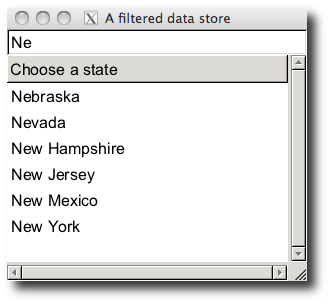
\includegraphics[width=.45\textwidth]{ex-RGtk2-filtered}
  \caption{Example of a data store filtered by values typed into a
    text-entry widget.}
  \label{fig:RGtk2-filtered}
\end{figure}

First, we create a data frame. The
\code{VISIBLE} column will be added to the \code{rGtkDataFrame}
instance to adjust the visible rows.
\begin{Schunk}
\begin{Sinput}
 df <- data.frame(state.name)
 df$VISIBLE <- rep(TRUE, nrow(df))
 store <- rGtkDataFrame(df)
\end{Sinput}
\end{Schunk}

The filtered store needs to have the column specified that contains
the logical values; in this example, it is the last column.
\begin{Schunk}
\begin{Sinput}
 filteredStore <- store$filter()
 filteredStore$setVisibleColumn(ncol(df)-1)      # offset
 view <- gtkTreeView(filteredStore)
\end{Sinput}
\end{Schunk}

Next, we create a basic view of a single column:
\begin{Schunk}
\begin{Sinput}
 view$insertColumnWithAttributes(0, "Col", gtkCellRendererText(), text = 0)
\end{Sinput}
\begin{Soutput}
[1] 1
\end{Soutput}
\end{Schunk}

An entry widget will be used to control the filtering. In the
callback, we adjust the \code{VISIBLE} column of the
\code{rGtkDataFrame} instance to reflect the rows to be shown. When
\code{val} is an empty string, the result of \function{grepl} is 
\code{TRUE}, so all rows will be shown.
\begin{Schunk}
\begin{Sinput}
 e <- gtkEntry()
 gSignalConnect(e, "changed", function(w, data) {
   pattern <- w$getText()
   df <- data$getModel()
   values <- df[, "state.name"]
   df[, "VISIBLE"] <- grepl(pattern, values)
 }, data=filteredStore)
\end{Sinput}
\begin{Soutput}
changed 
    503 
attr(,"class")
[1] "CallbackID"
\end{Soutput}
\end{Schunk}


Figure~\ref{fig:RGtk2-filtered} shows the two widgets placed within a
simple GUI.
\end{example}

\subsection{Cell renderer details}
\label{sec:RGtk2:cellrenderers}

The values in a tree model are rendered in a rectangular cell by the
derivatives of \class{GtkCellRenderer}. Cell renderers are
interactive, in that they also manage editing and activation of cells.

A cell renderer is independent of any data model. Its rendering role
is limited to drawing into a specified rectangular region according to
its current property values. An object that implements the
\class{GtkCellLayout} interface, like \class{GtkTreeViewColumn} and
\class{GtkComboBox} (see Section~\ref{sec:RGtk2:mvc:combobox}),
associates a set of \emph{attributes} with a cell renderer. An
attribute is a link between an aesthetic property of a cell renderer
and a column in the data model. When the \class{GtkCellLayout} object
needs to render a particular cell, it configures the properties of the
renderer with the values from the current model row, according to the
attributes. Thus, the mapping from data to visualization depends on
the class of the renderer instance, its explicit property settings,
and the attributes associated with the renderer in the cell layout.

For example, to render text, a \class{GtkCellRendererText} is
appropriate. The \code{text} property is usually linked via an
attribute to a text column in the model, as the text would vary from
row to row. However, the background color (the \code{background}
property) might be common to all rows in the column and thus is set
explicitly, without use of an attribute.

%% TODO: put some sort of simple example code block here

The base class \class{GtkCellRenderer} defines a number of properties
that are common to all rendering tasks. The \code{xalign} and
\code{yalign} properties specify the alignment, i.e., how to position
the rendered region when it does not fill the entire cell. The
\code{cell-background} property indicates the color for the entire
cell background.

The rest of this section describes each type of cell renderer, as well
as some advanced features.

%% text/ numbers
\paragraph{Text cell renderers}

The \constructor{gtkCellRendererText} constructor is used to display
text and numeric values. Numeric values in the model are shown as
strings.  The most important property is \code{text}, the actual text
that is displayed. Other properties control the display of the text,
such as the font \code{family} and \code{size}, the \code{foreground}
and \code{background} colors, and whether to \code{ellipsize} or
\code{wrap} the text if there is not enough space for display.

To display right-aligned text in a Helvetica font, the following could be used:
\begin{Schunk}
\begin{Sinput}
 cr <- gtkCellRendererText()
 cr['xalign'] <- 1                       # default 0.5 = centered
 cr['family'] <- "Helvetica"  
\end{Sinput}
\end{Schunk}

The \code{wrap} attribute can be specified as \code{TRUE}, if the
entries are expected to be long. There are several other attributes that can
changed. 

When an attribute links the \code{text} property to a numeric column
in the model, the property system automatically converts the number to
its string representation. This occurs according to the same logic
that \R\/ follows to print numeric values, so options like
\code{scipen} and \code{digits} are considered. See the ``Overriding
attribute mappings'' paragraph below for further customization.

%% perhaps could be adapted to demonstrate the above
% \begin{example}{A basic usage of displaying a data frame using a tree view}{ex:RGtk2-minimal-rGtkDataFrame}
%   \SweaveInput{ex-RGtk2-minimal-rGtkDataFrame}
% \end{example}

%% combo
\paragraph{Editable text renderers}

\class{GtkCellRendererCombo} and \class{GtkCellRendererSpin} allow
editing a text cell with a combo box or spin button,
respectively. Populating the combo box menu requires specifying two
properties: \code{model} and \code{text-column}. The menu items are
retrieved from the \class{GtkTreeModel} given by \code{model} at the
column index given by \code{text-column}.  If \code{has-entry} is
\code{TRUE}, a combo box entry is displayed.
\begin{Schunk}
\begin{Sinput}
 cr <- gtkCellRendererCombo()
 store <- rGtkDataFrame(state.name)
 cr['model'] <- store
 cr['text-column'] <- 0
 cr['editable'] <- TRUE                  # needed
\end{Sinput}
\end{Schunk}
The spin button editor is configured by passing a
\class{GtkAdjustment} to the \code{adjustment} property.


%% pixbuf
\paragraph{Pixbuf cell renderers}

To display an image in a cell, \class{GtkCellRendererPixbuf} is
appropriate. The image is specified through one of its properties:
\code{stock-id}, a stock identifier; \code{icon-name}, the name of a
themed icon; or \code{pixbuf}, an actual \code{GdkPixbuf}
object. It is possible to store a \class{GdkPixbuf} in a
\class{data.frame}, and thus an \class{RGtkDataFrame}, using a \class{list}:
\begin{Schunk}
\begin{Sinput}
 library(RGtk2)
 apple <- gdkPixbuf(filename = imagefile("apple-red.png"))[[1]]
 floppy <- gdkPixbuf(filename = imagefile("floppybuddy.gif"))[[1]]
 logo <- gdkPixbuf(filename = imagefile("rgtk-logo.gif"))[[1]]
 rdf <- rGtkDataFrame(data.frame(image = I(list(apple, floppy, logo))))
 view <- gtkTreeView(rdf)
 view$insertColumnWithAttributes(0, "image", gtkCellRendererPixbuf(), pixbuf = 0)
\end{Sinput}
\begin{Soutput}
[1] 1
\end{Soutput}
\begin{Sinput}
 win <- gtkWindow()
 win$add(view)
\end{Sinput}
\end{Schunk}

%% ping pong
\begin{example}{A widget for variable selection}{ex:RGtk2-pingpong}
This example shows a combination widget that is familiar from other
statistics GUIs. It provides two tree views listing variable names and
has arrows to move variable names from one side to the other. Often
such widgets are used for specifying statistical models. 

\begin{figure}
  \centering
  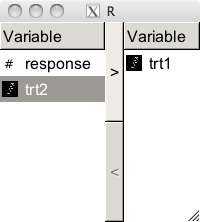
\includegraphics[width=.4\textwidth]{ex-RGtk2-pingpong}
  \caption{An example showing to tree views with buttons to move
    entries from one to the other. This is a common method for
    variable selection.}
  \label{fig:RGtk2-pingpong}
\end{figure}


We will use Example~\ref{ex:RGtk2:add-stock-icons}, in particular its
function \code{addToStockIcons}, to add some custom
stock icons to identify the variable type.
\begin{Schunk}
\begin{Sinput}
 fileNms <- c(factor = system.file("images","factor.gif", package="gWidgets"),
              numeric = system.file("images","numeric.gif", package="gWidgets"))
 pixbufs <- lapply(fileNms, function(fn) gdkPixbuf(file = fn)[[1]])
 addToStockIcons(pixbufs)
\end{Sinput}
\end{Schunk}

To keep track of the variables in the two tree views we use a single
model. It has a column for all the variable names, a column for the
icon, and two columns to keep track of which variable names are to be
displayed in the respective tree views.
\begin{Schunk}
\begin{Sinput}
 d <- data.frame(varNames=c("response", "trt1", "trt2"),
                 stock.id=c("new-numeric", "new-factor", "new-factor"),
                 leftView  = rep(TRUE, 3),
                 rightView = rep(FALSE, 3),
                 stringsAsFactors=FALSE)
 model <- rGtkDataFrame(d)
\end{Sinput}
\end{Schunk}

We will use a filtered data store to show each tree view.
As the two tree views are identical, except for the rows that are
displayed, we generate them with a function. The \code{vis.col}
indicates which column in the \code{rGtkDataFrame} object contains the
visibility information. Our tree view packs in both a pixbuf cell
renderer and a text cell renderer.
\begin{Schunk}
\begin{Sinput}
 makeView <- function(model, vis.col) {
   filteredModel <- model$filter()
   filteredModel$setVisibleColumn(vis.col - 1)
   tv <- gtkTreeView(filteredModel)
   tv$getSelection()$setMode("multiple")
   ##
   cr <- gtkCellRendererPixbuf()
   cr['xalign'] <- 1
   tv$insertColumnWithAttributes(0, "Variable", cr, "stock-id" = 1)
   vc <- tv$getColumn(0)
   ##
   cr <- gtkCellRendererText()
   vc$PackStart(cr, expand=TRUE)
   cr['xalign'] <- 0
   cr['xpad'] <- 5
   vc$addAttribute(cr, "text", 0)
 
   return(tv)
 }
\end{Sinput}
\end{Schunk}
We now create the tree views:
\begin{Schunk}
\begin{Sinput}
 views <- list()
 views[["left"]] <- makeView(model,3)
 views[["right"]] <- makeView(model,4)
 selections <- lapply(views, gtkTreeViewGetSelection)
\end{Sinput}
\end{Schunk}
We need buttons to move the values left and right; these are stored
in a list for convenience.
\begin{Schunk}
\begin{Sinput}
 buttons <- list()
 buttons[["fromLeft"]] <- gtkButton(">")
 buttons[["fromRight"]] <- gtkButton("<")
\end{Sinput}
\end{Schunk}

Our basic GUI is shown in Figure~\ref{fig:RGtk2-pingpong} where the
two tree views are placed side-by-side.
%The basic GUI just lays out the two tree views with the buttons in
%between. We left out command to add scrollwindows etc.

The key handler moves the selected value from one side to the other. A
complication is that when the view is using filtering the selection
returns values relative to the child model (the filtered one). In
general, the methods \code{convertChildPathToPath} and
\code{convertChildIterToIter} of the filtered model will translate
between the two models, but in this case we map the indices using the
appropriate visibility column. This handler assumes that an index
indicating the view (\code{i}) is passed as user data.
\begin{Schunk}
\begin{Sinput}
 moveSelected <- function(b, i) {
   selection <- selections[[i]]
   selected <- selection$getSelectedRows()
   if(length(selected$retval)) {
     childRows <- sapply(selected$retval, function(childPath) {
       childRow <- as.numeric(childPath$toString()) + 1L
     })
     shownIndices <- which(model[, 2L + i])
     rows <- shownIndices[childRows]
     
     model[rows, 2L + i] <- FALSE
     model[rows, 2L + (3L-i)] <- !model[rows, 2L + i]
   }
 }
\end{Sinput}
\end{Schunk}
We connect the handler to the \qcode{clicked} signal for the buttons.
\begin{Schunk}
\begin{Sinput}
 mapply(gSignalConnect, buttons, "clicked", list(moveSelected), 1:2)
\end{Sinput}
\begin{Soutput}
 fromLeft.clicked fromRight.clicked 
              588               589 
\end{Soutput}
\end{Schunk}

We add one flourish, namely ensuring that the arrows are not sensitive
when the corresponding selection is not set.
\begin{Schunk}
\begin{Sinput}
 disableButton <- function(sel, button) {
   selected <- sel$getSelectedRows()
   button$setSensitive(length(selected$retval) != 0)
 }
 mapply(gSignalConnect, selections, "changed", list(disableButton), buttons)
\end{Sinput}
\begin{Soutput}
 left.changed right.changed 
          590           591 
\end{Soutput}
\end{Schunk}
%
As the initial state has no selection, we set the button
sensitivities accordingly.
\begin{Schunk}
\begin{Sinput}
 sapply(buttons, gtkWidgetSetSensitive, FALSE)
\end{Sinput}
\begin{Soutput}
$fromLeft
NULL

$fromRight
NULL
\end{Soutput}
\end{Schunk}
\end{example}

\paragraph{Toggle cell renderers}

Binary data can be represented by a toggle. The
\constructor{gtkCellRendererToggle} will create a check box in the
cell that will appear checked if the \code{active} property is
\code{TRUE}. If an attribute is defined for the property, then changes
in the model will be reflected in the view. More work is required to
modify the model in response to user interaction with the view. The
\code{activatable} attribute for the cell must be \code{TRUE} in order
for it to receive user input. The programmer needs to connect to the
\signal{toggled} to update the model in response to changes in the
active state.
\begin{Schunk}
\begin{Sinput}
 cr <- gtkCellRendererToggle()
 cr['activatable'] <- TRUE               # cell can be activated
 cr['active'] <- TRUE
 gSignalConnect(cr, "toggled", function(w, path) {
   model$active[as.numeric(path) + 1] <- w['active']
 })
\end{Sinput}
\begin{Soutput}
toggled 
    593 
attr(,"class")
[1] "CallbackID"
\end{Soutput}
\end{Schunk}

To render the toggle as a radio button instead of a check box, set the
\code{radio} property to \code{TRUE}. The programmer is responsible
for implementing the radio button logic via the \code{toggled} signal.

\begin{example}{Displaying a check box column in a tree
    view}{ex:RGtk2-add-toggle-to-df}
This example demonstrates the construction of a GUI for selecting one
or more rows from a data frame. We will display a list of the installed
packages that can be upgraded from CRAN, although this code is
trivially generalizable to any list of choices. The user selects a row
by clicking on a checkbox produced by a toggle cell renderer.


To get the installed packages that can be upgraded, we use some of the
functions provided by the  \pkg{utils} package.
\begin{Schunk}
\begin{Sinput}
 d <- old.packages()[,c("Package", "Installed", "ReposVer")]
 d <- as.data.frame(d)
\end{Sinput}
\end{Schunk}


This function will be called on the selected rows. Here, we simply
call \function{install.packages} to update the selected packages.
\begin{Schunk}
\begin{Sinput}
 doUpdate <- function(d) {
   install.packages(d$Package)
 }
\end{Sinput}
\end{Schunk}

To display the data frame, we first append a column to the data frame
to store the selection information and then create a corresponding
\class{RGtkDataFrame}.
\begin{Schunk}
\begin{Sinput}
 n <- ncol(d)
 nms <- colnames(d)
 d$.toggle <- rep(FALSE, nrow(d))
 store <- rGtkDataFrame(d)
\end{Sinput}
\end{Schunk}

Our tree view shows each text column using a simple text cell renderer,
except for the first column that contains the check boxes for selection.
\begin{Schunk}
\begin{Sinput}
 view <- gtkTreeView()
 # add toggle
 cr <- gtkCellRendererToggle()
 view$insertColumnWithAttributes(0, "", cr, active = n)
\end{Sinput}
\begin{Soutput}
[1] 1
\end{Soutput}
\begin{Sinput}
 cr['activatable'] <- TRUE
 gSignalConnect(cr, "toggled", function(cr, path, user.data) {
   view <- user.data
   row <- as.numeric(path) + 1
   model <- view$getModel()
   n <- dim(model)[2]
   model[row, n] <- !model[row, n]
 }, data=view)
\end{Sinput}
\begin{Soutput}
toggled 
    610 
attr(,"class")
[1] "CallbackID"
\end{Soutput}
\end{Schunk}

The text columns are added one-by-one in a similar manner:

\begin{Schunk}
\begin{Sinput}
 mapply(view$insertColumnWithAttributes, -1, nms, list(gtkCellRendererText()), 
        text = 1:n-1)
\end{Sinput}
\begin{Soutput}
[1] 2 3 4
\end{Soutput}
\end{Schunk}

Finally, we connect the store to the model.
\begin{Schunk}
\begin{Sinput}
 view$setModel(store)
\end{Sinput}
\end{Schunk}

To allow the user to initiate the action, we create a button and
assign a callback. We pass in the view, rather than the model, in case
the model would be recreated by the \code{doUpdate} call. In a real
application, once a package is upgraded it would be removed from the
display.
\begin{Schunk}
\begin{Sinput}
 b <- gtkButton("Update packages")
 gSignalConnect(b, "clicked", function(w, data) {
   view <- data
   model <- view$getModel()
   n <- dim(model)[2]
   vals <- model[model[, n], -n, drop=FALSE]
   doUpdate(vals)
 }, data=view)
\end{Sinput}
\begin{Soutput}
clicked 
    633 
attr(,"class")
[1] "CallbackID"
\end{Soutput}
\end{Schunk}


Our basic GUI places the view into a box container that also holds the
button to initiate the action.
\begin{Schunk}
\begin{Sinput}
 w <- gtkWindow(show=FALSE)
 w$setTitle("Installed packages that need upgrading")
 w$setSizeRequest(300, 300)
 g <- gtkVBox(); w$add(g)
 sw <- gtkScrolledWindow()
 g$packStart(sw, expand=TRUE, fill=TRUE)
 sw$add(view)
 sw$setPolicy("automatic", "automatic")
 g$packStart(b, expand=FALSE)
 w$show()
\end{Sinput}
\end{Schunk}
\end{example}

%% progress bars
\paragraph{Rendering progress in cells}

To visually communicate progress within a cell, both progress bars and
spinner animations are supported. These modes correspond to
\class{GtkCellRendererProgress} and \class{GtkCellRendererSpinner},
respectively.

In the case of \class{GtkCellRendererProgress}, its \code{value}
property takes a value between $0$ and $100$ indicating the amount
finished, with a default value of $0$. Values out of this range will
be signaled by an error message.  The \code{orientation} property,
with values from \code{GtkProgressBarOrientation}, can adjust the
direction that the bar grows.  For example,

\begin{Schunk}
\begin{Sinput}
 cr <- gtkCellRendererProgress()
 cr["value"] <- 50                       # fixed 50%
 cr['orientation'] <- "right-to-left"
\end{Sinput}
\end{Schunk}

For indicating progress in the absence of a definite end point,
\class{GtkCellRendererSpinner} is more appropriate. The spinner is
displayed when the \code{active} property is \code{TRUE}. Increment
the \code{pulse} property to drive the animation.

%% numbers
\paragraph{Overriding attribute mappings}

The default behavior for mapping model values to a renderer property
is simple: values are extracted from the model and passed directly to
the cell renderer property. If the data types are different, such as a
numeric value for a string property, the value is converted using
low-level routines defined by the property system. It is sometimes desirable to override this mapping with more complex logic.

For example, conversion of numbers to strings is a non-trivial
task. Although the logic in the \R\/ print system often performs
acceptably, there is certainly room for customization, for example
aligning floating point numbers by fixing the number of decimal
places. This could be done in the model (e.g., using
\function{sprintf} to format and coerce to character data). However,
performing the conversion during rendering requires one to to
intercept the model value before it is passed to the cell renderer. In
the specific case \class{GtkTreeView}, it is possible to specify a
callback that overrides this step.  

The callback, of type \class{GtkTreeCellDataFunc}, accepts arguments
for the tree view column, the cell renderer, the model, an iterator
pointing to the row in the model and an argument for user data. The
function is tasked with setting the appropriate attributes of the cell
renderer. For example, this function could be used to format floating
point numbers:
\begin{Schunk}
\begin{Sinput}
 func <- function(viewCol, cellRend, model, iter, data) {
   curVal <- model$getValue(iter, 0)$value
   fVal <- sprintf("%.3f", curVal)
   cellRend['text'] <- fVal
   cellRend['xalign'] <- 1
 }
\end{Sinput}
\end{Schunk}
%
The function then needs to be registered with a
\class{GtkTreeViewColumn} that is rendering a numeric column from the model:
\begin{Schunk}
\begin{Sinput}
 view <- gtkTreeView(rGtkDataFrame(data.frame(rnorm(100))))
 cr <- gtkCellRendererText()
 view$insertColumnWithAttributes(0, "numbers", cr, text = 0)
\end{Sinput}
\begin{Soutput}
[1] 1
\end{Soutput}
\begin{Sinput}
 vc <- view$getColumn(0)
 vc$setCellDataFunc(cr, func)
\end{Sinput}
\begin{Soutput}
NULL
\end{Soutput}
\end{Schunk}
%
The last line is the key: calling
\method{setCellDataFunc}{GtkTreeViewColumn} registers our custom
formatting function with the view column.

One drawback with the use of such functions is that \R\/ code is
executed every time a cell is rendered. If performance matters,
consider pre-converting the data in the model or tweaking the
\code{options} in \R\/ for printing real numbers, namely \code{scipen}
and \code{digits}.

For customizing rendering further and outside the scope of
\class{GtkTreeView}, one could implement a new type of
\class{GtkCellRenderer}. See Section~\ref{sec:rgtk2:extending-classes} for
more details on this advanced concept.

%% This function will be set for the tree view column and illustrated in Example~\ref{ex:RGtk2:rGtk2DataFrame}.
%% editable cells 

\paragraph{Editable cells} When the \code{editable} property of a text
cell (or \code{activatable} property of a toggle cell) is set to
\code{TRUE}, then the cell contents can be changed. This allows the
user to make changes to the underlying model through the GUI. Although
the view automatically reflects changes made to the model, the reverse
is not true. A callback must be assigned to the \code{editable}
(\code{toggled}) signal for the cell renderer to implement the
change. The callback for the \qcode{edited} signal has arguments
\code{renderer}, \code{path} for the path of the selected row (as a
string), and \code{new.text} containing the value of the edited text
as a string. The tree view object and which column was edited are not
passed in by default. These can be passed through the user data
argument, set as user data on the renderer, or accessed from an
enclosing environment if needed within the callback.

For example, here is how one can update an \code{RGtkDataFrame} model
from within the callback.
\begin{Schunk}
\begin{Sinput}
 cr['editable'] <- TRUE
 ID <- gSignalConnect(cr, "edited", 
 f=function(cr, path, newtext, user.data) {
   curRow <- as.numeric(path) + 1
   curCol <- user.data$column
   model <- user.data$model
   model[curRow, curCol] <- newtext
 }, data=list(model=store, column=1))
\end{Sinput}
\end{Schunk}

\paragraph{Moving the cursor}

Users may expect that once a cell is edited, the next cell is then set
up to be edited. In order to do this, one must advance the cursor and
activate editing of the next cell. For \class{GtkTreeView}, this is
done through the \method{setCursor}{gtkTreeView} method. The
\code{path} argument takes a tree path instance, the \code{column}
argument a tree view column object, and the flag \code{start.editing}
indicates whether to initiate editing.

% <<CellRendererExample>>=
% cr <- gtkCellRendererText()
% cr['family'] <- "Helvetica"             # font family for whole column
% cr['background'] <- "goldenrod"         # background color for column
% crp <- gtkCellRendererPixbuf();         # a pixbuf
% crp['xalign'] <- 0
% @

% Cellrenderers define how data is to be displayed. The binding of the
% data to the cell renderer is handled by the view, not the
% cellrenderer.

\section{Display of hierarchical data}
\label{sec:RGtk2:mvc:GtkTreeStore}

Although the \code{RGtkDataFrame} model is a convenient implementation
of \class{GtkTreeModel}, it has its limitations. Primary among them is
its lack of support for hierarchical data. \GTK\/ implements
\class{GtkTreeModel} with \class{GtkListStore} and
\class{GtkTreeStore}, which respectively store non-hierarchical and
hierachical tabular data. \class{GtkListStore} is a flat table,
while \class{GtkTreeStore} organizes the table into a hierarchy. Here,
we discuss \class{GtkTreeStore}.

\subsection{Loading hierarchical data}
  
%% ML: I'm pretty sure that RGtkDataFrame will support the same types
%% of values as GtkListStore. It's just a little tricky to get a
%% column of GdkPixbuf externalptr's into a data.frame. Much easier to
%% use a character vector and associate it with the stock.id property
%% of GtkCellRendererPixbuf, as long as the images are registered icons.

%% construction
A tree store is constructed using \constructor{gtkTreeStore}. The
column types are specified through a character vector at the time of
construction. The specification uses ``GTypes'' such as
\code{gchararray} for character data, \code{gboolean} for logical
data, \code{gint} for integer data, \code{gdouble} for numeric data,
and \code{GObject} for \GTK\/ objects, such as pixbufs.

\begin{example}{Defining a tree}{eg:RGtk2:tree-store}
  Below, we create a tree based on the \code{Cars93} dataset, where
  the car models are organized by manufacturer, i.e., each model row
  is the child of its manufacturer row:
\begin{Schunk}
\begin{Sinput}
 tstore <- gtkTreeStore("gchararray")
 by(Cars93, Cars93$Manufacturer, function(df) {
   piter <- tstore$append()              # parent
   tstore$setValue(piter$iter, column = 0, value = df$Manufacturer[1])
   sapply(df$Model, function(model) {
     sibiter <- tstore$append(parent = piter$iter) # child
     if (is.null(sibiter$retval)) 
       tstore$setValue(sibiter$iter, column = 0, value = model)
   })
 })
\end{Sinput}
\begin{Soutput}
Cars93$Manufacturer: Acura
[[1]]
NULL

[[2]]
NULL

------------------------------------------------------------ 
Cars93$Manufacturer: Audi
[[1]]
NULL

[[2]]
NULL

------------------------------------------------------------ 
Cars93$Manufacturer: BMW
[[1]]
NULL

------------------------------------------------------------ 
Cars93$Manufacturer: Buick
[[1]]
NULL

[[2]]
NULL

[[3]]
NULL

[[4]]
NULL

------------------------------------------------------------ 
Cars93$Manufacturer: Cadillac
[[1]]
NULL

[[2]]
NULL

------------------------------------------------------------ 
Cars93$Manufacturer: Chevrolet
[[1]]
NULL

[[2]]
NULL

[[3]]
NULL

[[4]]
NULL

[[5]]
NULL

[[6]]
NULL

[[7]]
NULL

[[8]]
NULL

------------------------------------------------------------ 
Cars93$Manufacturer: Chrylser
[[1]]
NULL

------------------------------------------------------------ 
Cars93$Manufacturer: Chrysler
[[1]]
NULL

[[2]]
NULL

------------------------------------------------------------ 
Cars93$Manufacturer: Dodge
[[1]]
NULL

[[2]]
NULL

[[3]]
NULL

[[4]]
NULL

[[5]]
NULL

[[6]]
NULL

------------------------------------------------------------ 
Cars93$Manufacturer: Eagle
[[1]]
NULL

[[2]]
NULL

------------------------------------------------------------ 
Cars93$Manufacturer: Ford
[[1]]
NULL

[[2]]
NULL

[[3]]
NULL

[[4]]
NULL

[[5]]
NULL

[[6]]
NULL

[[7]]
NULL

[[8]]
NULL

------------------------------------------------------------ 
Cars93$Manufacturer: Geo
[[1]]
NULL

[[2]]
NULL

------------------------------------------------------------ 
Cars93$Manufacturer: Honda
[[1]]
NULL

[[2]]
NULL

[[3]]
NULL

------------------------------------------------------------ 
Cars93$Manufacturer: Hyundai
[[1]]
NULL

[[2]]
NULL

[[3]]
NULL

[[4]]
NULL

------------------------------------------------------------ 
Cars93$Manufacturer: Infiniti
[[1]]
NULL

------------------------------------------------------------ 
Cars93$Manufacturer: Lexus
[[1]]
NULL

[[2]]
NULL

------------------------------------------------------------ 
Cars93$Manufacturer: Lincoln
[[1]]
NULL

[[2]]
NULL

------------------------------------------------------------ 
Cars93$Manufacturer: Mazda
[[1]]
NULL

[[2]]
NULL

[[3]]
NULL

[[4]]
NULL

[[5]]
NULL

------------------------------------------------------------ 
Cars93$Manufacturer: Mercedes-Benz
[[1]]
NULL

[[2]]
NULL

------------------------------------------------------------ 
Cars93$Manufacturer: Mercury
[[1]]
NULL

[[2]]
NULL

------------------------------------------------------------ 
Cars93$Manufacturer: Mitsubishi
[[1]]
NULL

[[2]]
NULL

------------------------------------------------------------ 
Cars93$Manufacturer: Nissan
[[1]]
NULL

[[2]]
NULL

[[3]]
NULL

[[4]]
NULL

------------------------------------------------------------ 
Cars93$Manufacturer: Oldsmobile
[[1]]
NULL

[[2]]
NULL

[[3]]
NULL

[[4]]
NULL

------------------------------------------------------------ 
Cars93$Manufacturer: Plymouth
[[1]]
NULL

------------------------------------------------------------ 
Cars93$Manufacturer: Pontiac
[[1]]
NULL

[[2]]
NULL

[[3]]
NULL

[[4]]
NULL

[[5]]
NULL

------------------------------------------------------------ 
Cars93$Manufacturer: Saab
[[1]]
NULL

------------------------------------------------------------ 
Cars93$Manufacturer: Saturn
[[1]]
NULL

------------------------------------------------------------ 
Cars93$Manufacturer: Subaru
[[1]]
NULL

[[2]]
NULL

[[3]]
NULL

------------------------------------------------------------ 
Cars93$Manufacturer: Suzuki
[[1]]
NULL

------------------------------------------------------------ 
Cars93$Manufacturer: Toyota
[[1]]
NULL

[[2]]
NULL

[[3]]
NULL

[[4]]
NULL

------------------------------------------------------------ 
Cars93$Manufacturer: Volkswagen
[[1]]
NULL

[[2]]
NULL

[[3]]
NULL

[[4]]
NULL

------------------------------------------------------------ 
Cars93$Manufacturer: Volvo
[[1]]
NULL

[[2]]
NULL
\end{Soutput}
\end{Schunk}
  To retrieve a value from the tree store using its path we have:
\begin{Schunk}
\begin{Sinput}
 iter <- tstore$getIterFromString("0:0")
 tstore$getValue(iter$iter, column = 0)$value
\end{Sinput}
\begin{Soutput}
[1] "Integra"
\end{Soutput}
\end{Schunk}
This obtains the first model from the first manufacturer.

\end{example}

As shown in this example, populating a tree store relies on two
functions: \method{append}{GtkTreeStore}, for appending rows, and
\method{setValue}{GtkTreeStore}, for setting row values. The iterator
to the parent row is passed to \method{append}{GtkTreeStore}. A parent
of \code{NULL}, the default, indicates that the row should be at the
top level. It would also be possible to insert rows using
\method{insert}{GtkTreeStore}, \method{insertBefore}{GtkTreeStore}, or
\method{insertAfter}{GtkTreeStore}. The
\method{setValue}{GtkTreeStore} method expects the row iterator and
the column index, $0$-based.

An entire row can be assigned through the \method{set}{gtkTreeStore}
method. The method uses positional arguments to specify the column and
the value. The column index appears as an even argument (say $2k$) and
the corresponding value in the odd argument (say $2k+1$).  Values are
returned by the \method{getValue}{gtkListStore} method, in a list with
component \code{value} storing the value.

Traversing a tree store is most easily achieved through the user of
\Rclass{GtkTreeIter}, introduced previously in the context of flat
tables. Here we perform a depth-first traversal of our \code{Cars93}
model to obtain the model values: 
\begin{Schunk}
\begin{Sinput}
 iter <- tstore$getIterFirst()
 models <- NULL
 flag <- iter$retval
 while(flag) {
   child <- tstore$iterChildren(iter$iter)
   while(child$retval) {
     models <- c(models, tstore$get(child$iter, 0)[[1]])
   }
   flag <- tstore$iterNext(iter$iter)
 }